\begin{figure}[H]
\centering
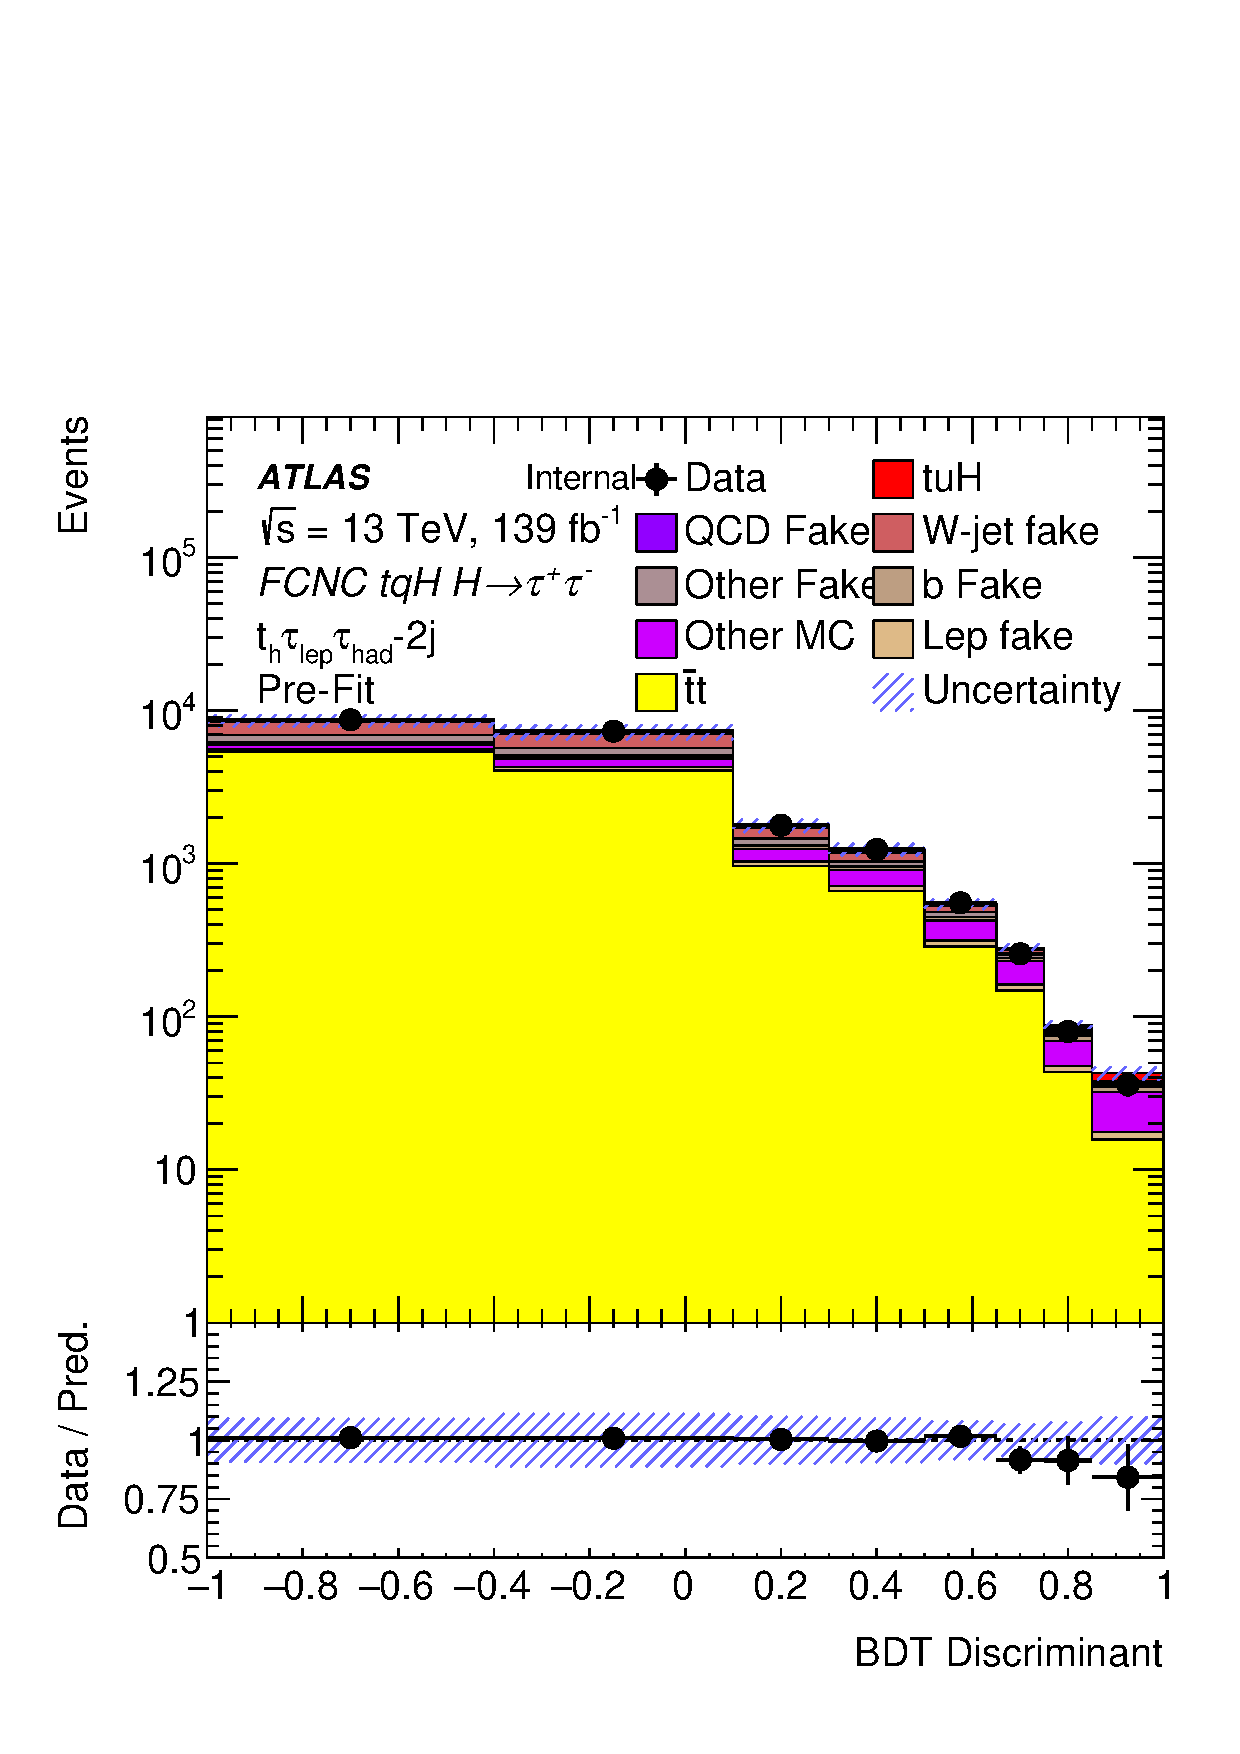
\includegraphics[width=0.40\textwidth]{\FCNCFigures/unblinded/ttHML/tuH_reg1l1tau1b2j_os.pdf}
\put(-100, 55){\textbf{(a1)}}
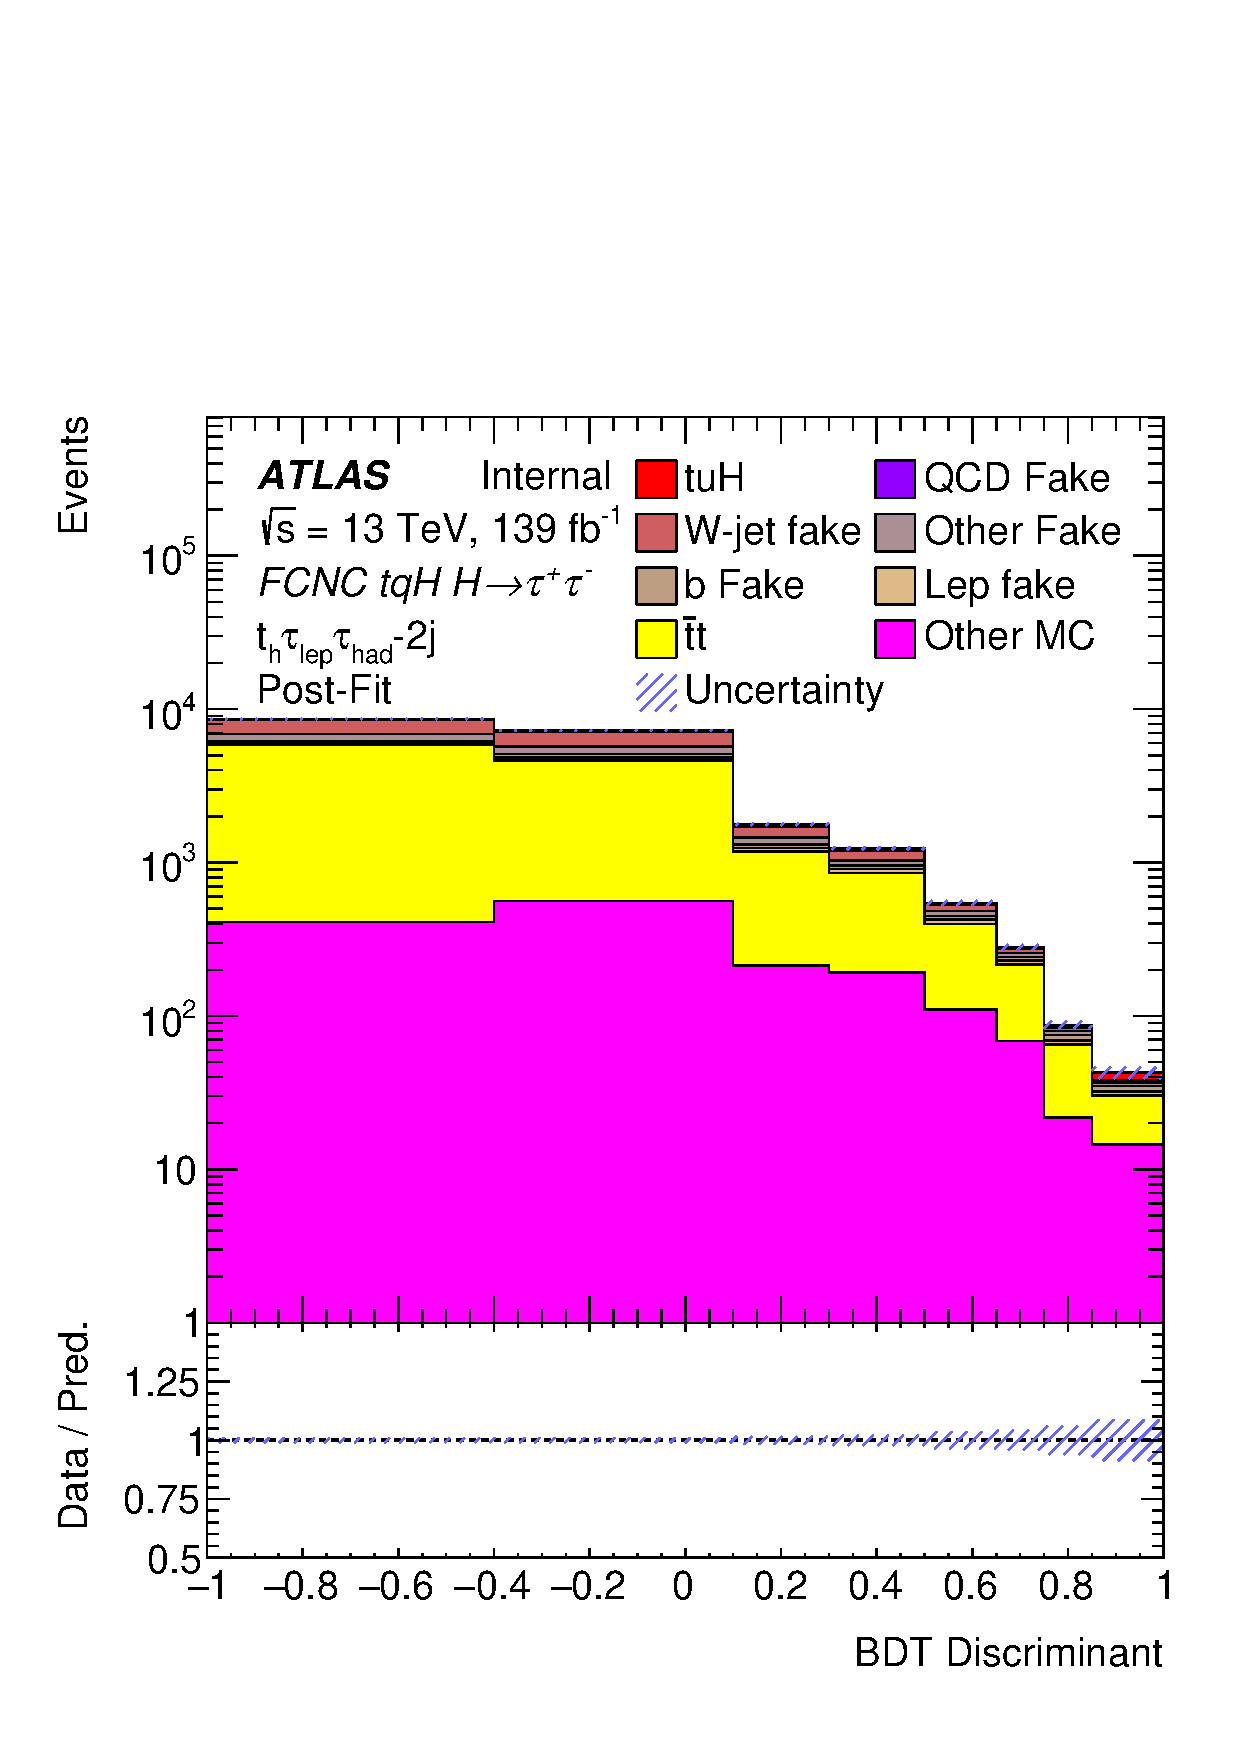
\includegraphics[width=0.40\textwidth]{\FCNCFigures/unblinded/ttHML/tuH_reg1l1tau1b2j_os_postFit.pdf}
\put(-100, 55){\textbf{(a2)}}\\
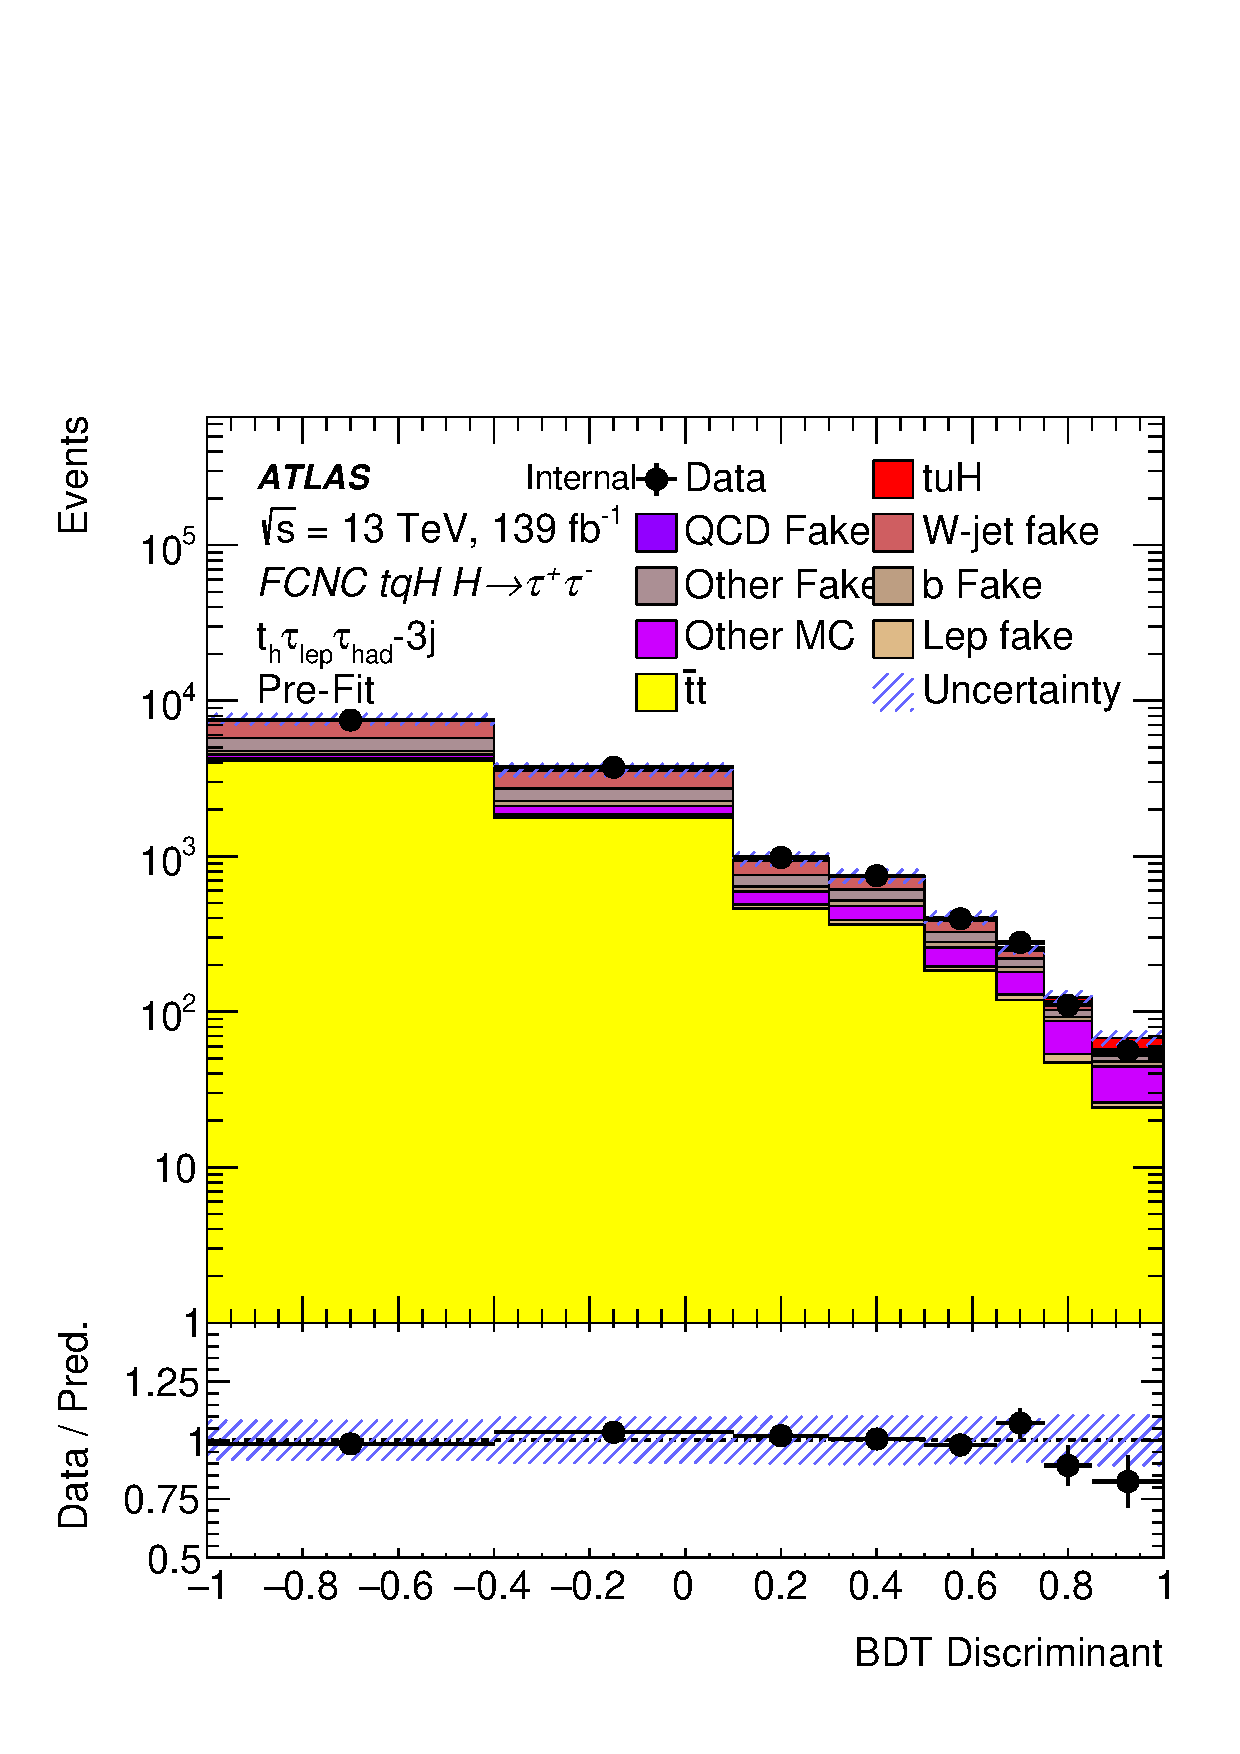
\includegraphics[width=0.40\textwidth]{\FCNCFigures/unblinded/ttHML/tuH_reg1l1tau1b3j_os.pdf}
\put(-100, 55){\textbf{(b1)}}
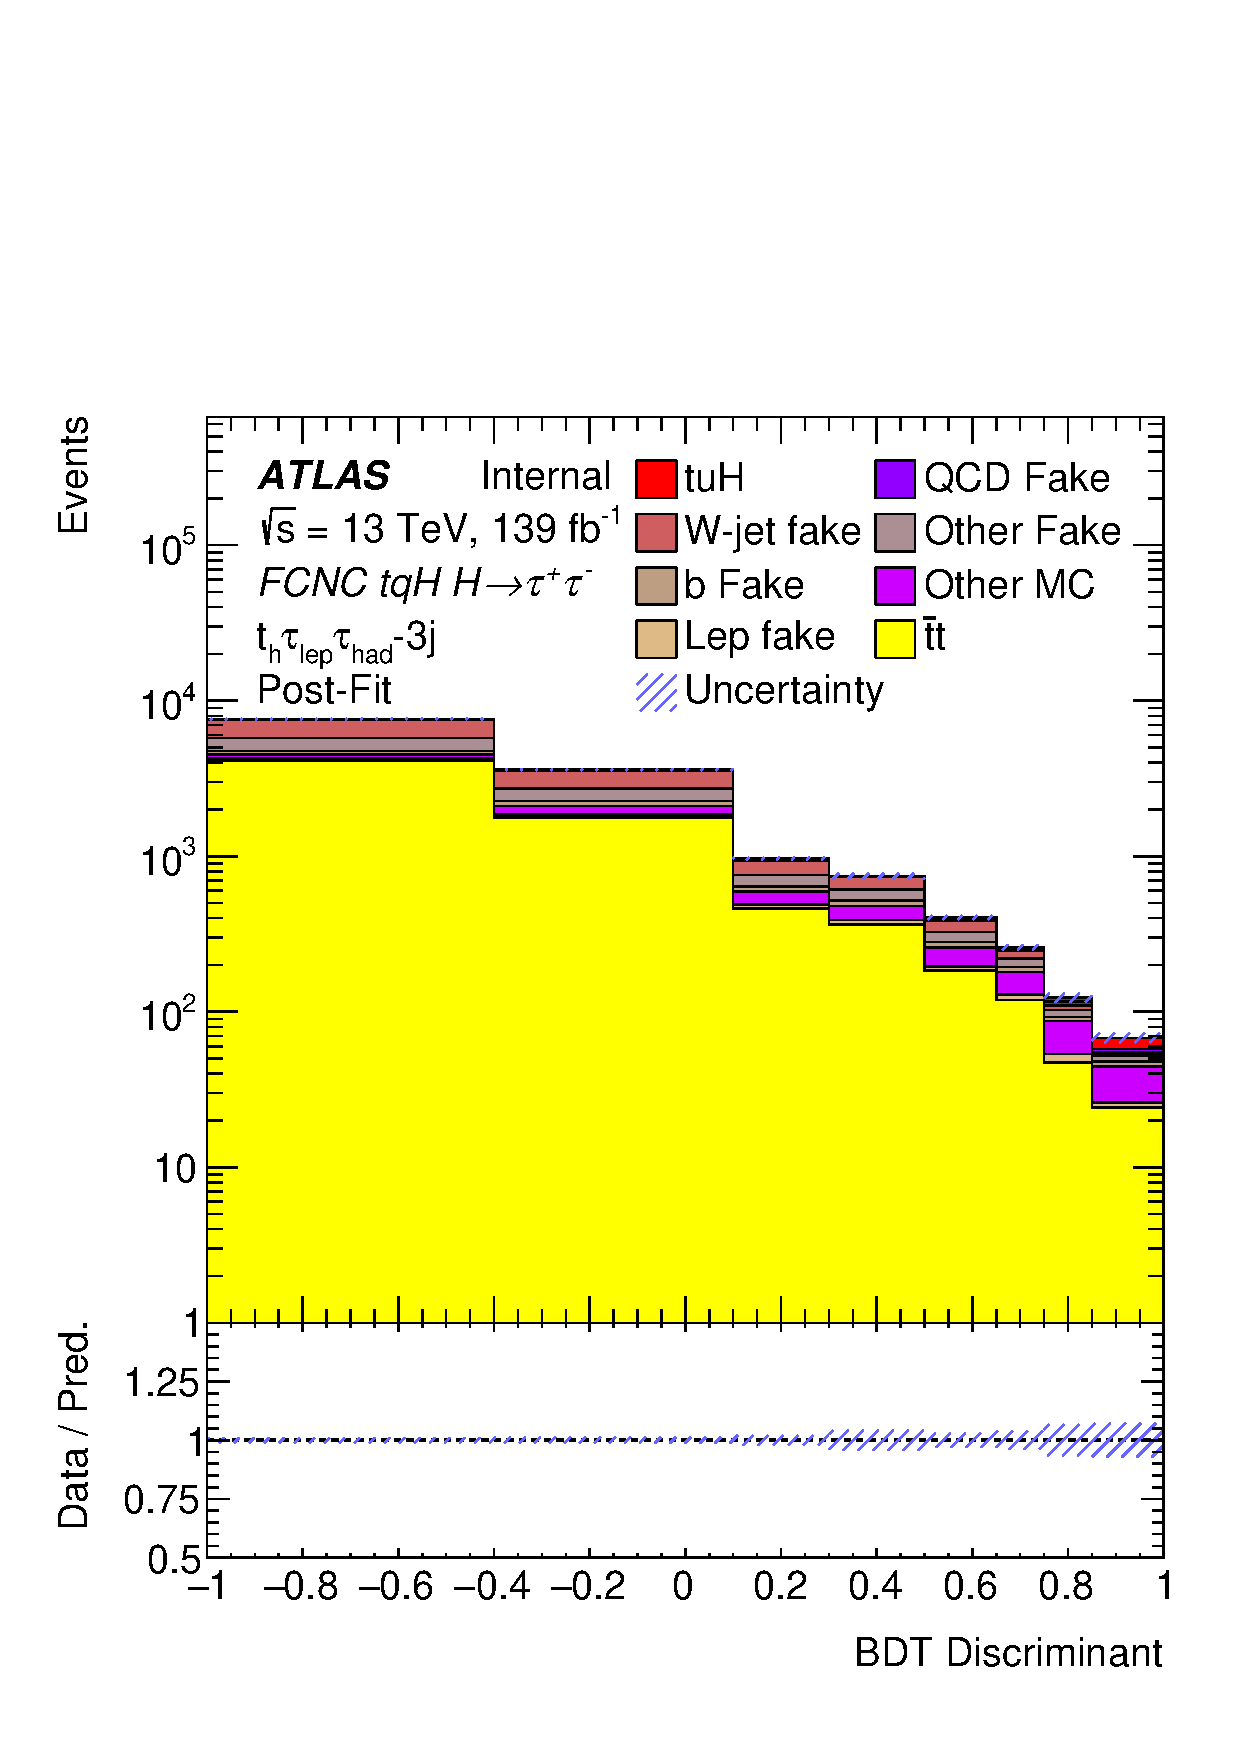
\includegraphics[width=0.40\textwidth]{\FCNCFigures/unblinded/ttHML/tuH_reg1l1tau1b3j_os_postFit.pdf}
\put(-100, 55){\textbf{(b2)}}\\
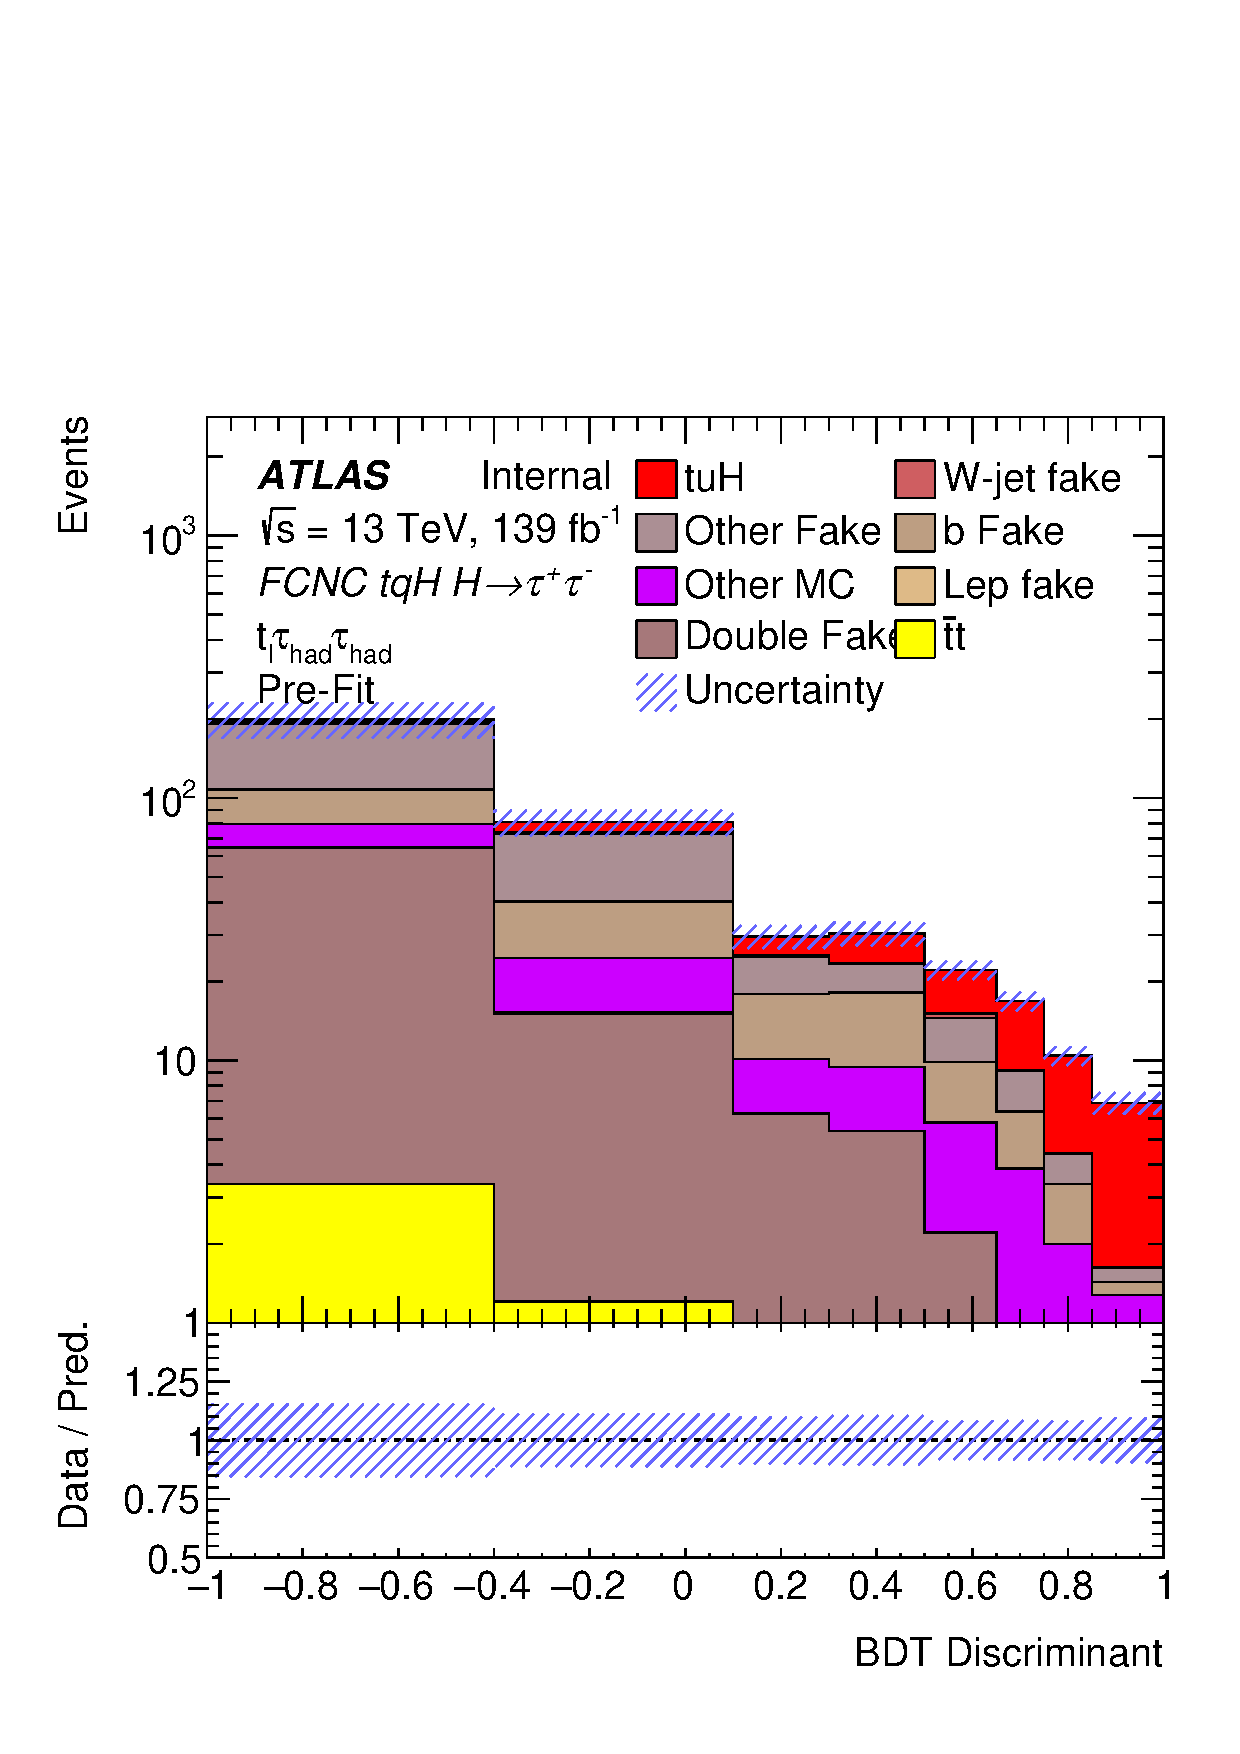
\includegraphics[width=0.40\textwidth]{\FCNCFigures/unblinded/ttHML/tuH_reg1l2tau1bnj_os.pdf}
\put(-100, 55){\textbf{(c1)}}
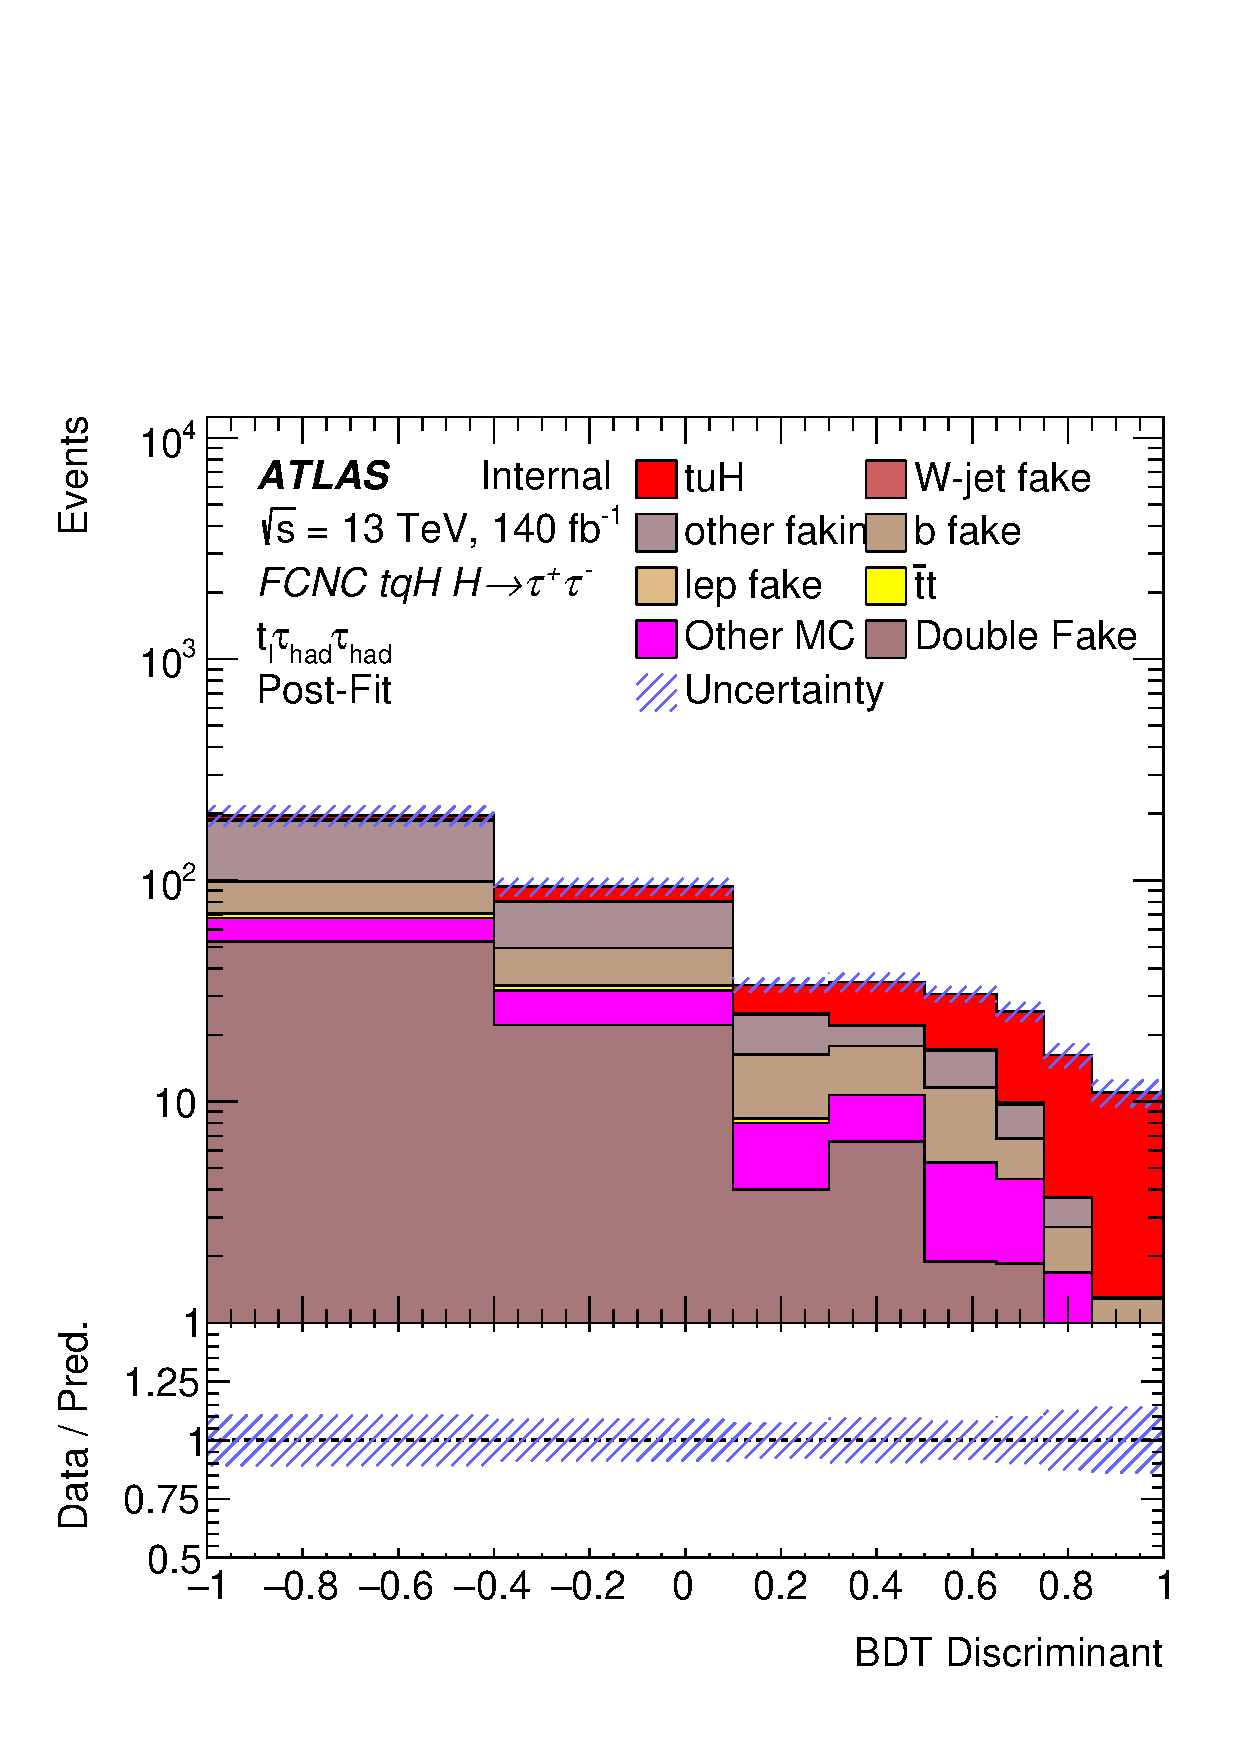
\includegraphics[width=0.40\textwidth]{\FCNCFigures/unblinded/ttHML/tuH_reg1l2tau1bnj_os_postFit.pdf}
\put(-100, 55){\textbf{(c2)}}\\

\caption{ Comparison of the shape of the BDT discriminant distribution between the unblinded prefit (a1,b1), unblinded postfit(a2,b2) in terms of tuH merged signal. The upper two plots are in the  $t_h\tlhad$-2j (a1-a2) region, the medium two are in $t_h\tlhad$-3j (b1-b2) and the bottom two are in $t_l\thadhad$ (c1-c2) . Statistical and systematic uncertainties are being shown.}
\label{fig:tthML_trexPrefit}
\end{figure}

\begin{figure}[H]
\centering
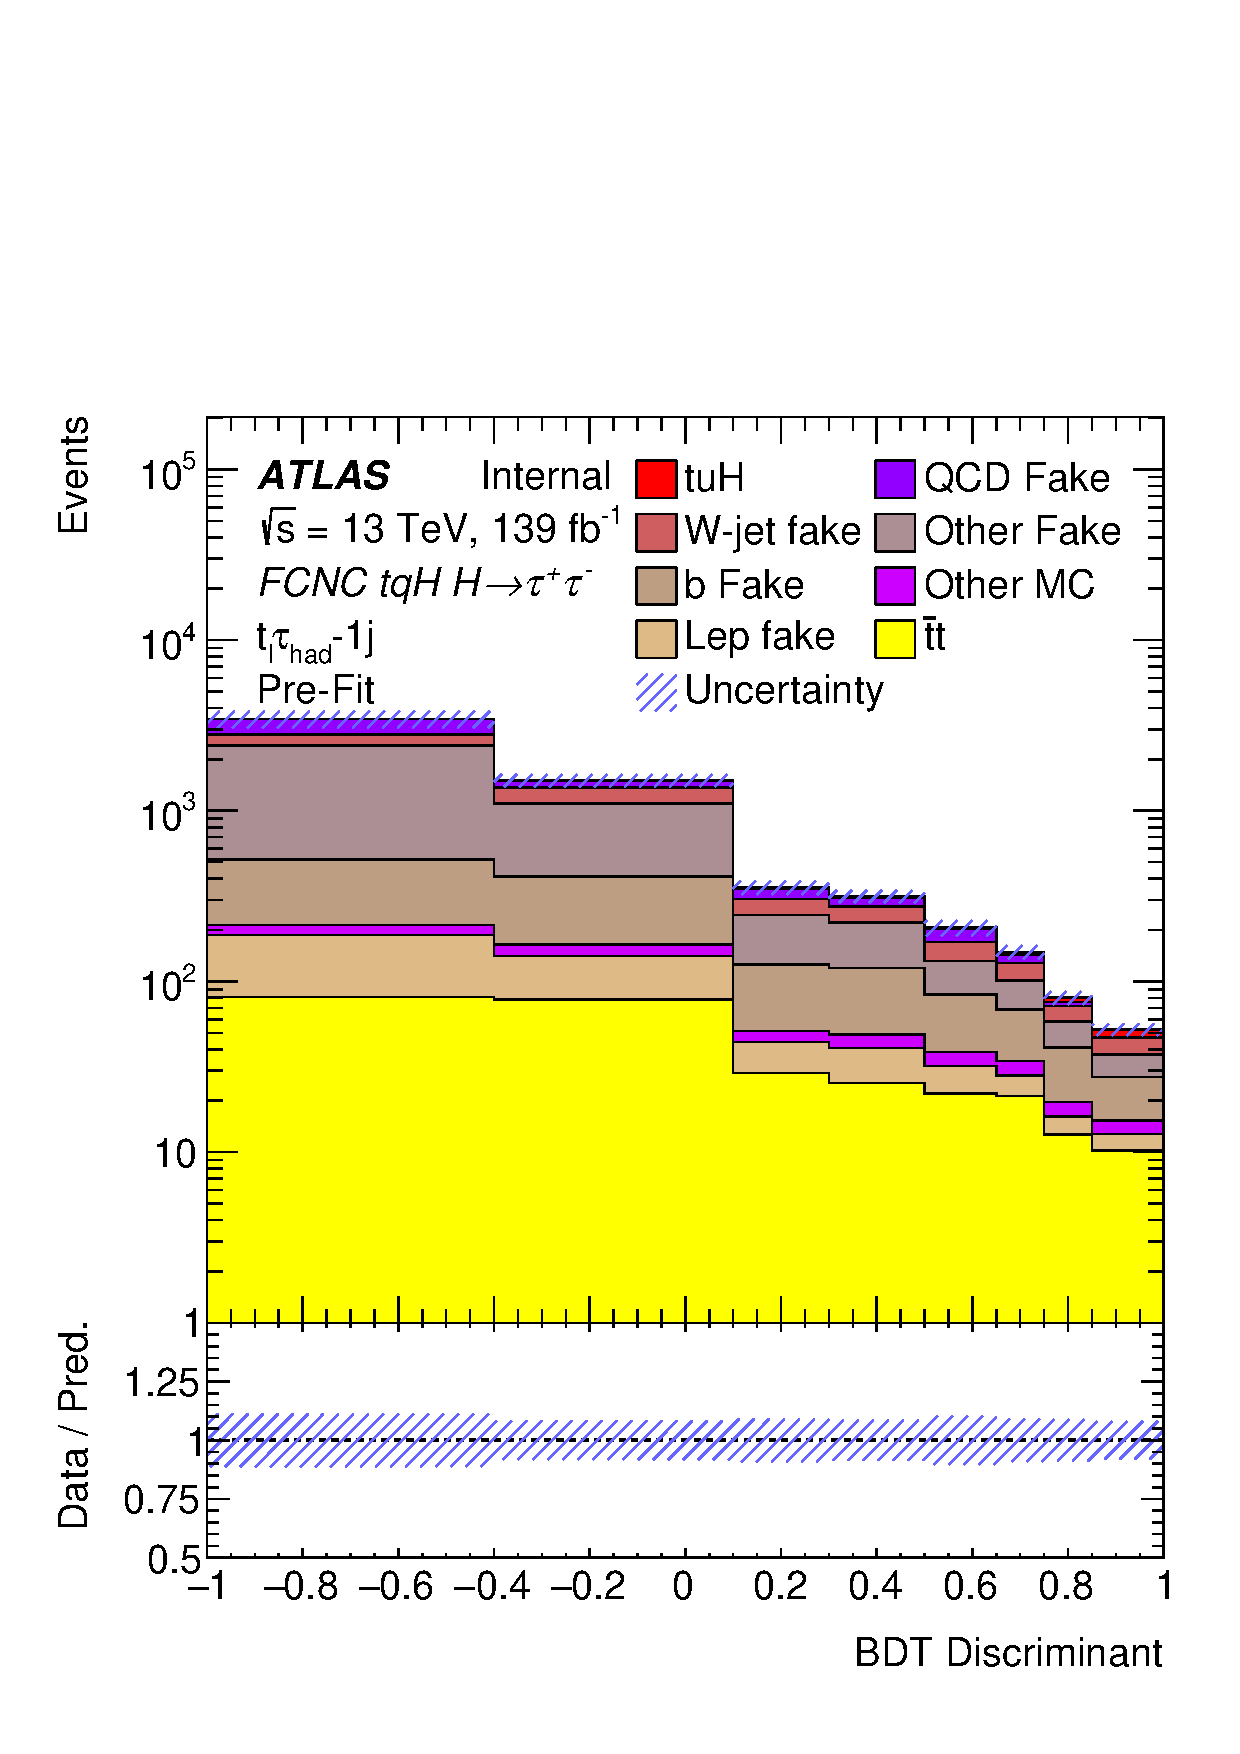
\includegraphics[width=0.50\textwidth]{\FCNCFigures/unblinded/ttHML/tuH_reg1l1tau1b1j_ss.pdf}
\put(-100, 55){\textbf{(a1)}}
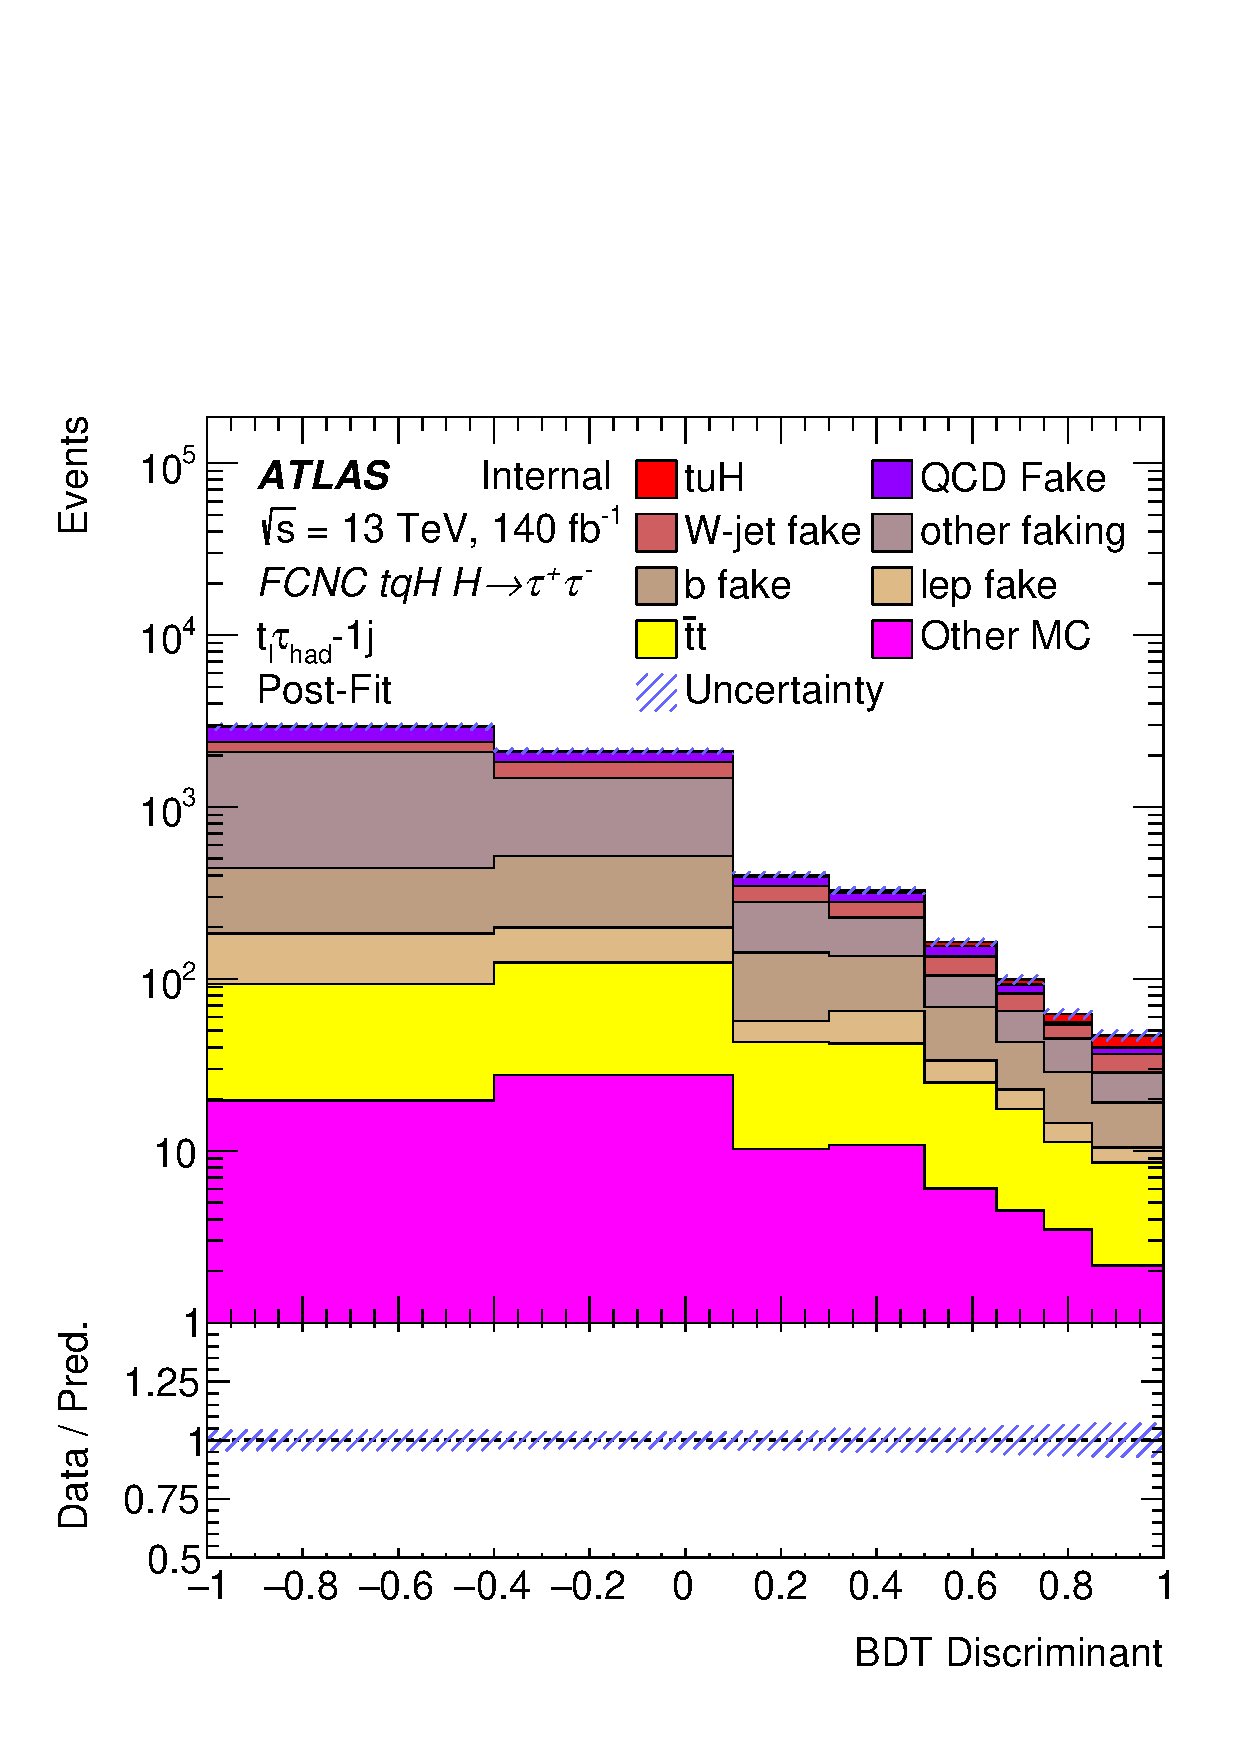
\includegraphics[width=0.50\textwidth]{\FCNCFigures/unblinded/ttHML/tuH_reg1l1tau1b1j_ss_postFit.pdf}
\put(-100, 55){\textbf{(a2)}}\\
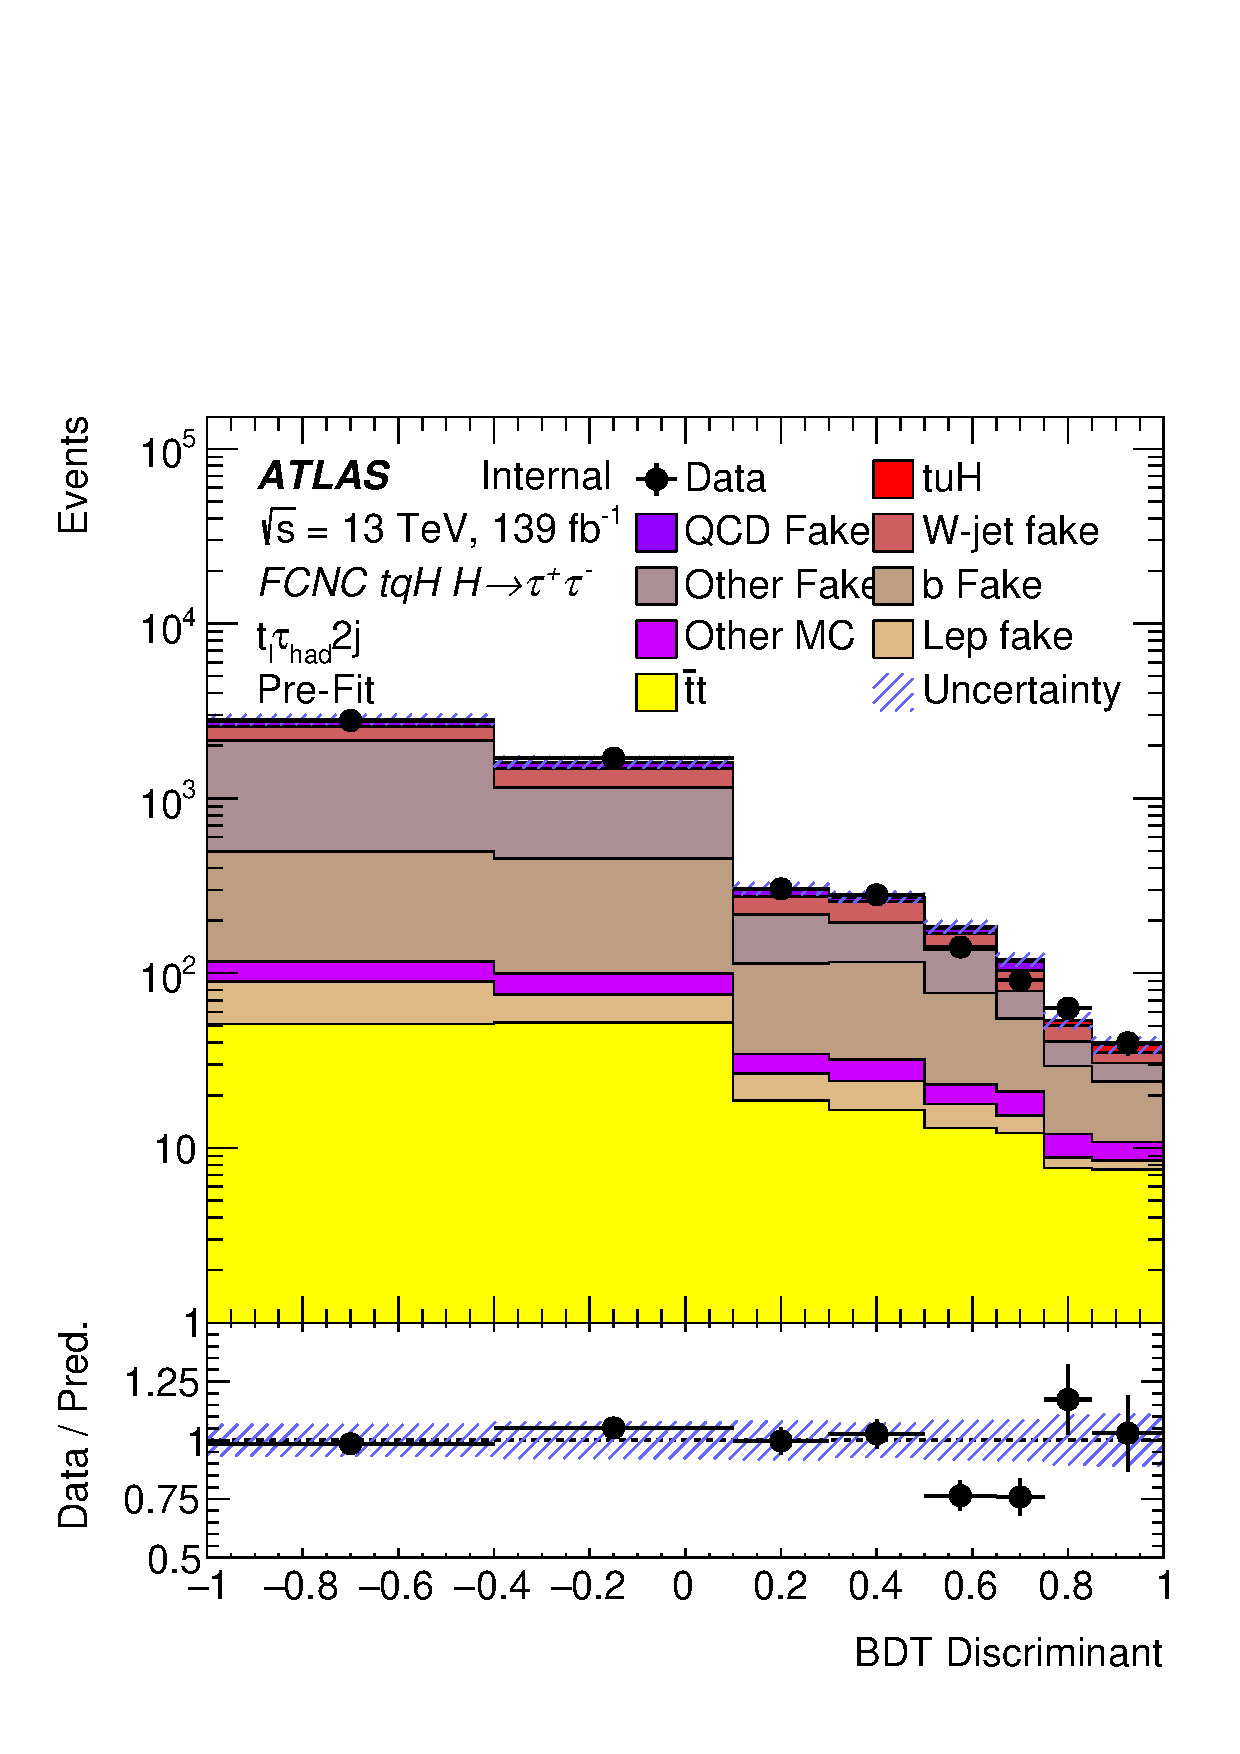
\includegraphics[width=0.50\textwidth]{\FCNCFigures/unblinded/ttHML/tuH_reg1l1tau1b2j_ss.pdf}
\put(-100, 55){\textbf{(b1)}}
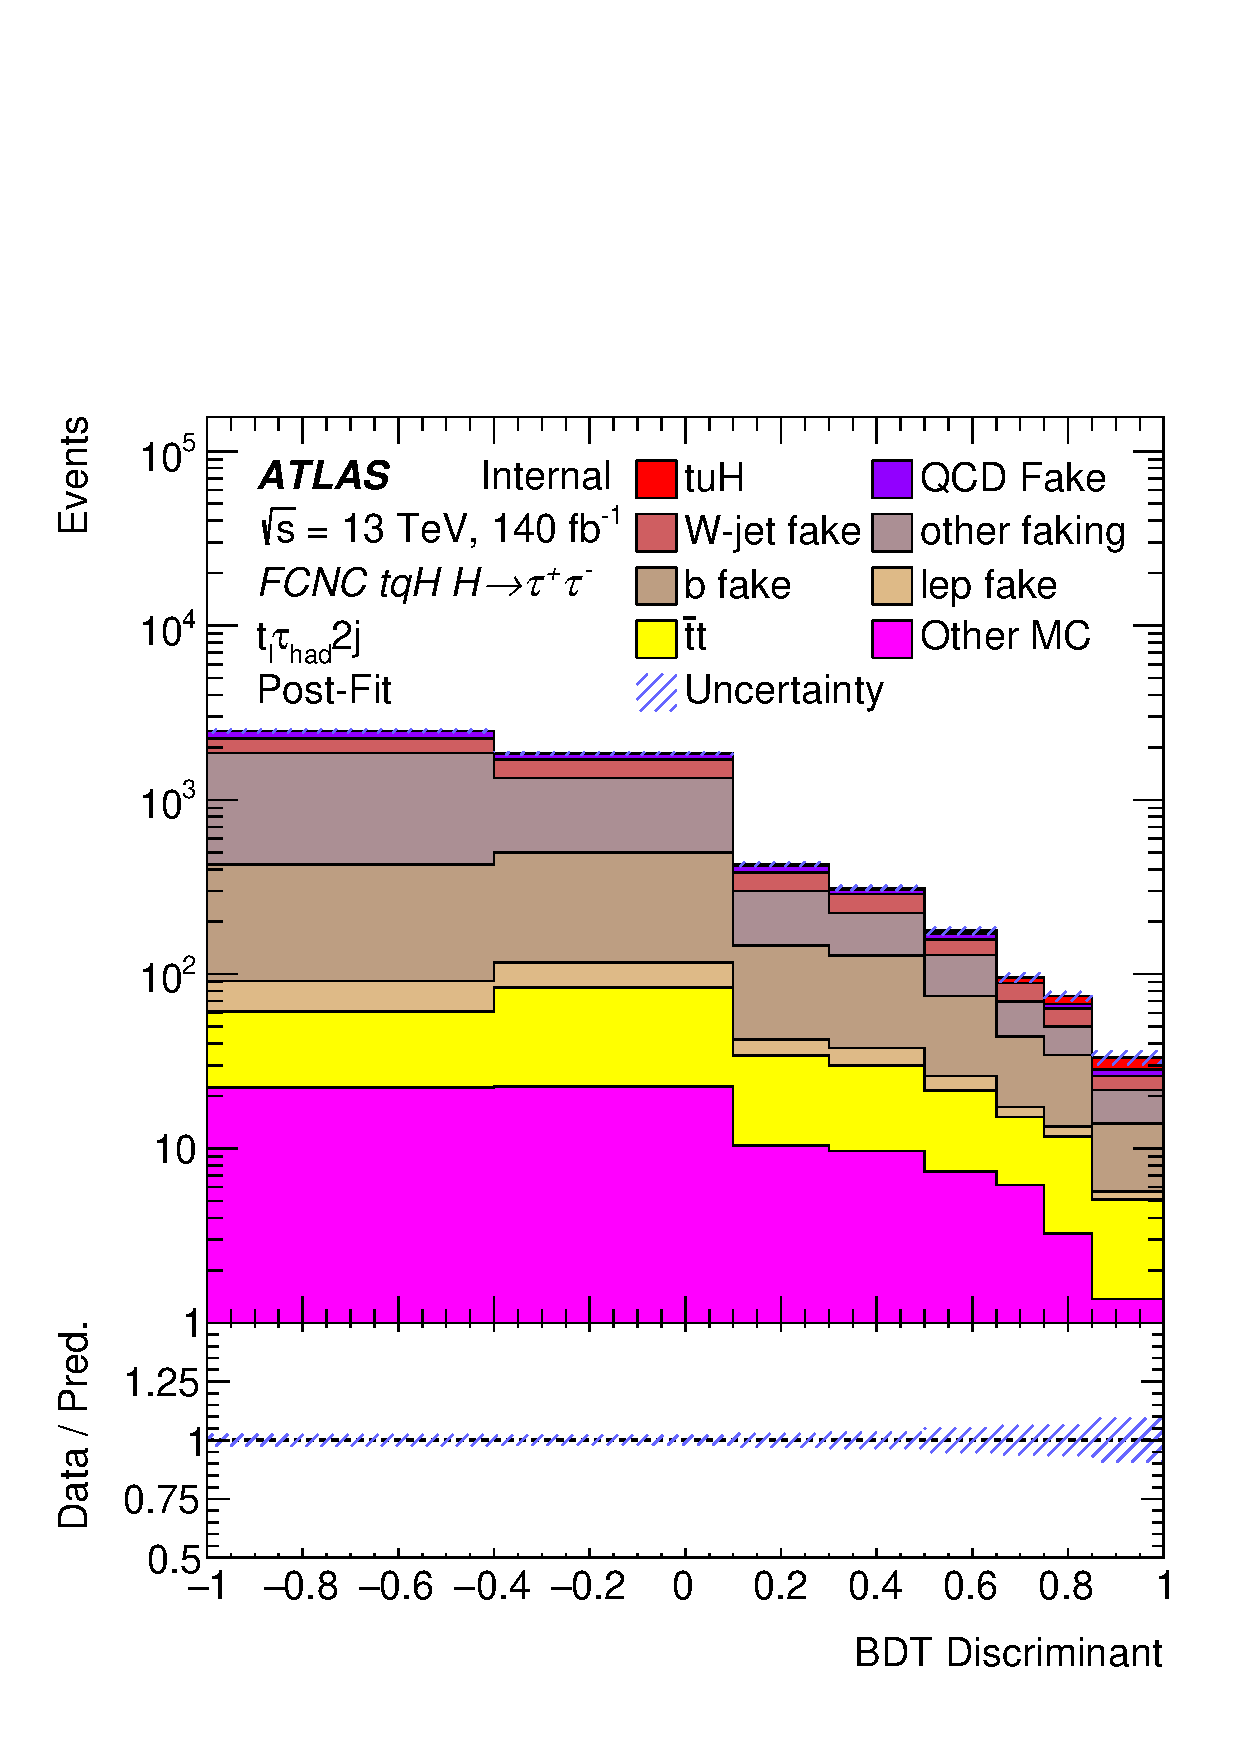
\includegraphics[width=0.50\textwidth]{\FCNCFigures/unblinded/ttHML/tuH_reg1l1tau1b2j_ss_postFit.pdf}
\put(-100, 55){\textbf{(b2)}}\\

\caption{ Comparison of the shape of the BDT discriminant distribution between the unblinded prefit (a1,b1), unblinded postfit (a2,b2) in terms of tuH merged signal.The upper two plots are in the  $t_l\tauhad$-1j (a1-a2) region, and the bottom two are in $t_l\tauhad$-2j (b1-b2).Statistical and systematic uncertainties are being shown.}
\label{fig:tthML_trexPrefit_1}
\end{figure}

\begin{figure}[H]
\centering
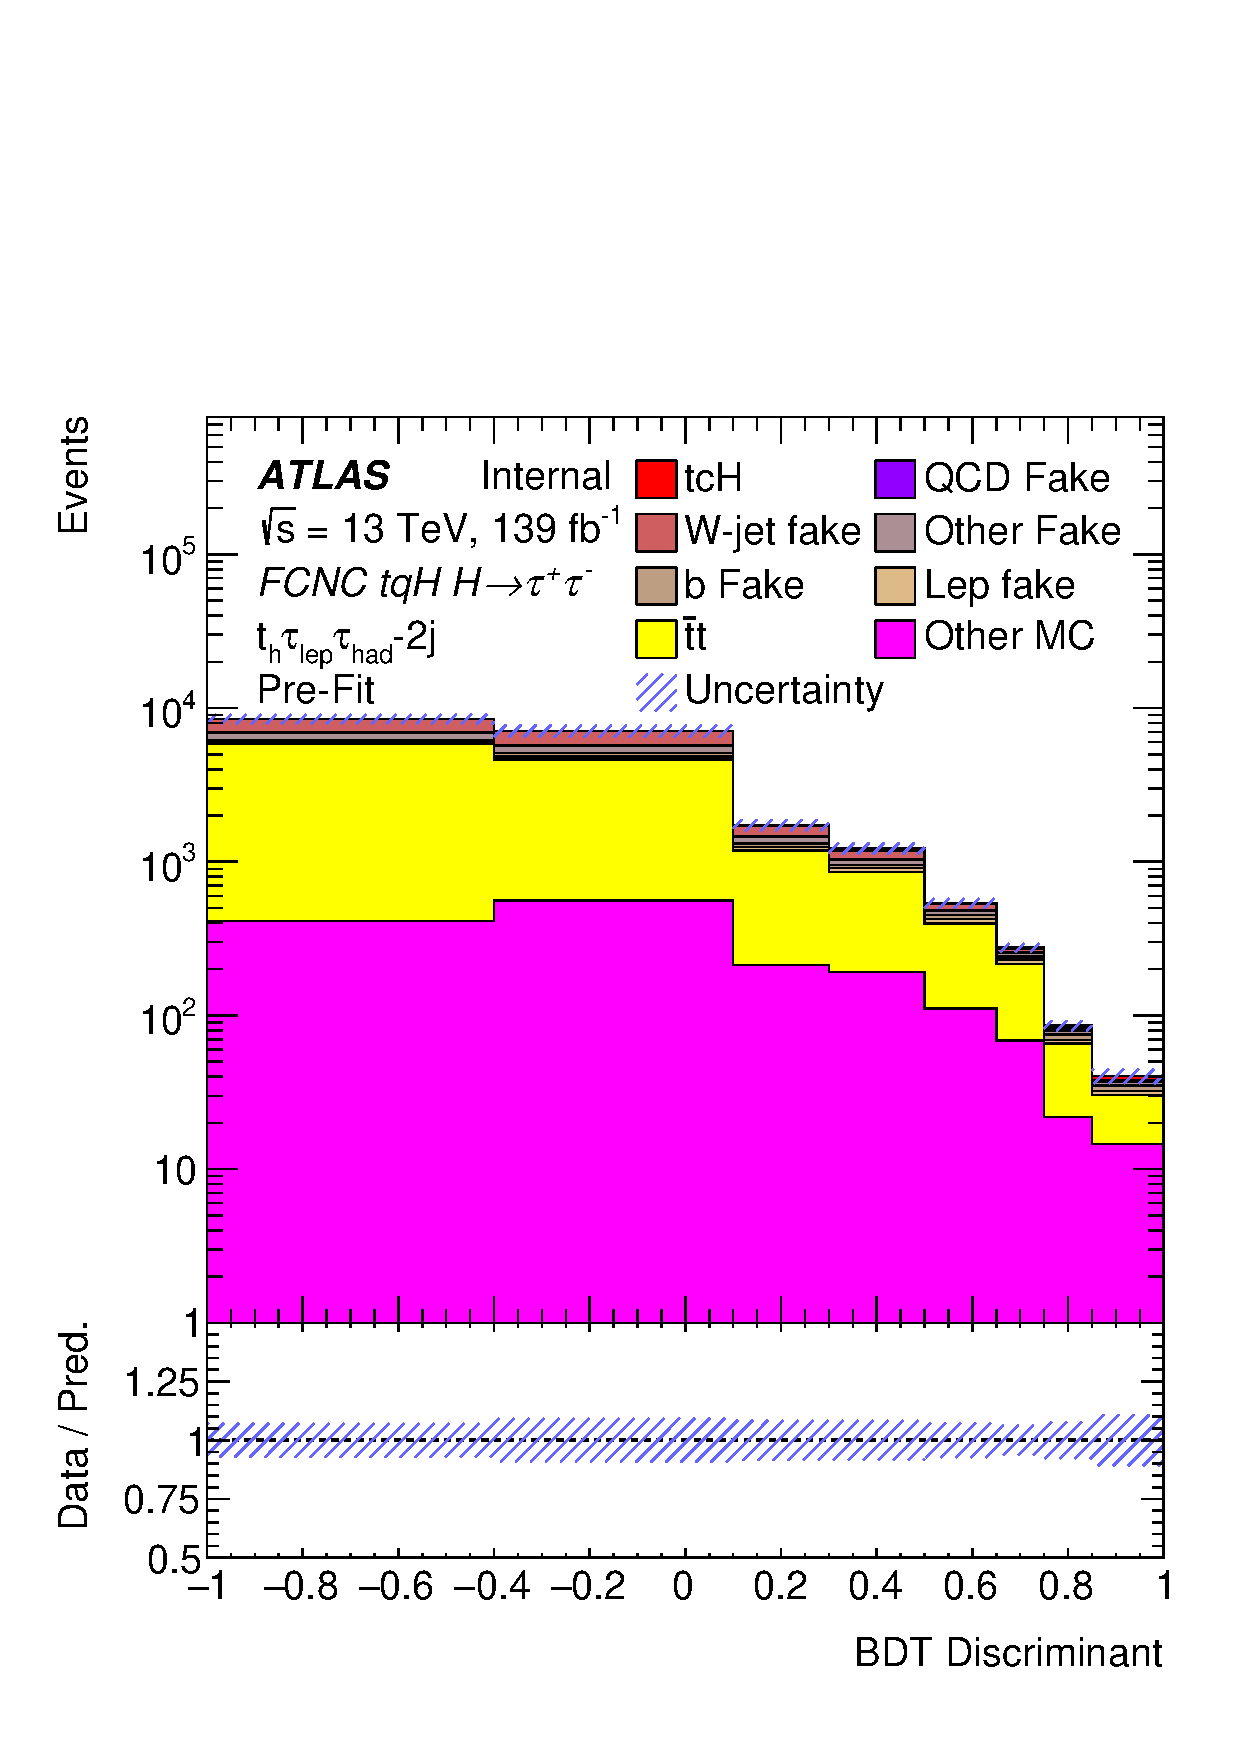
\includegraphics[width=0.40\textwidth]{\FCNCFigures/unblinded/ttHML/tcH_reg1l1tau1b2j_os.pdf}
\put(-100, 55){\textbf{(a1)}}
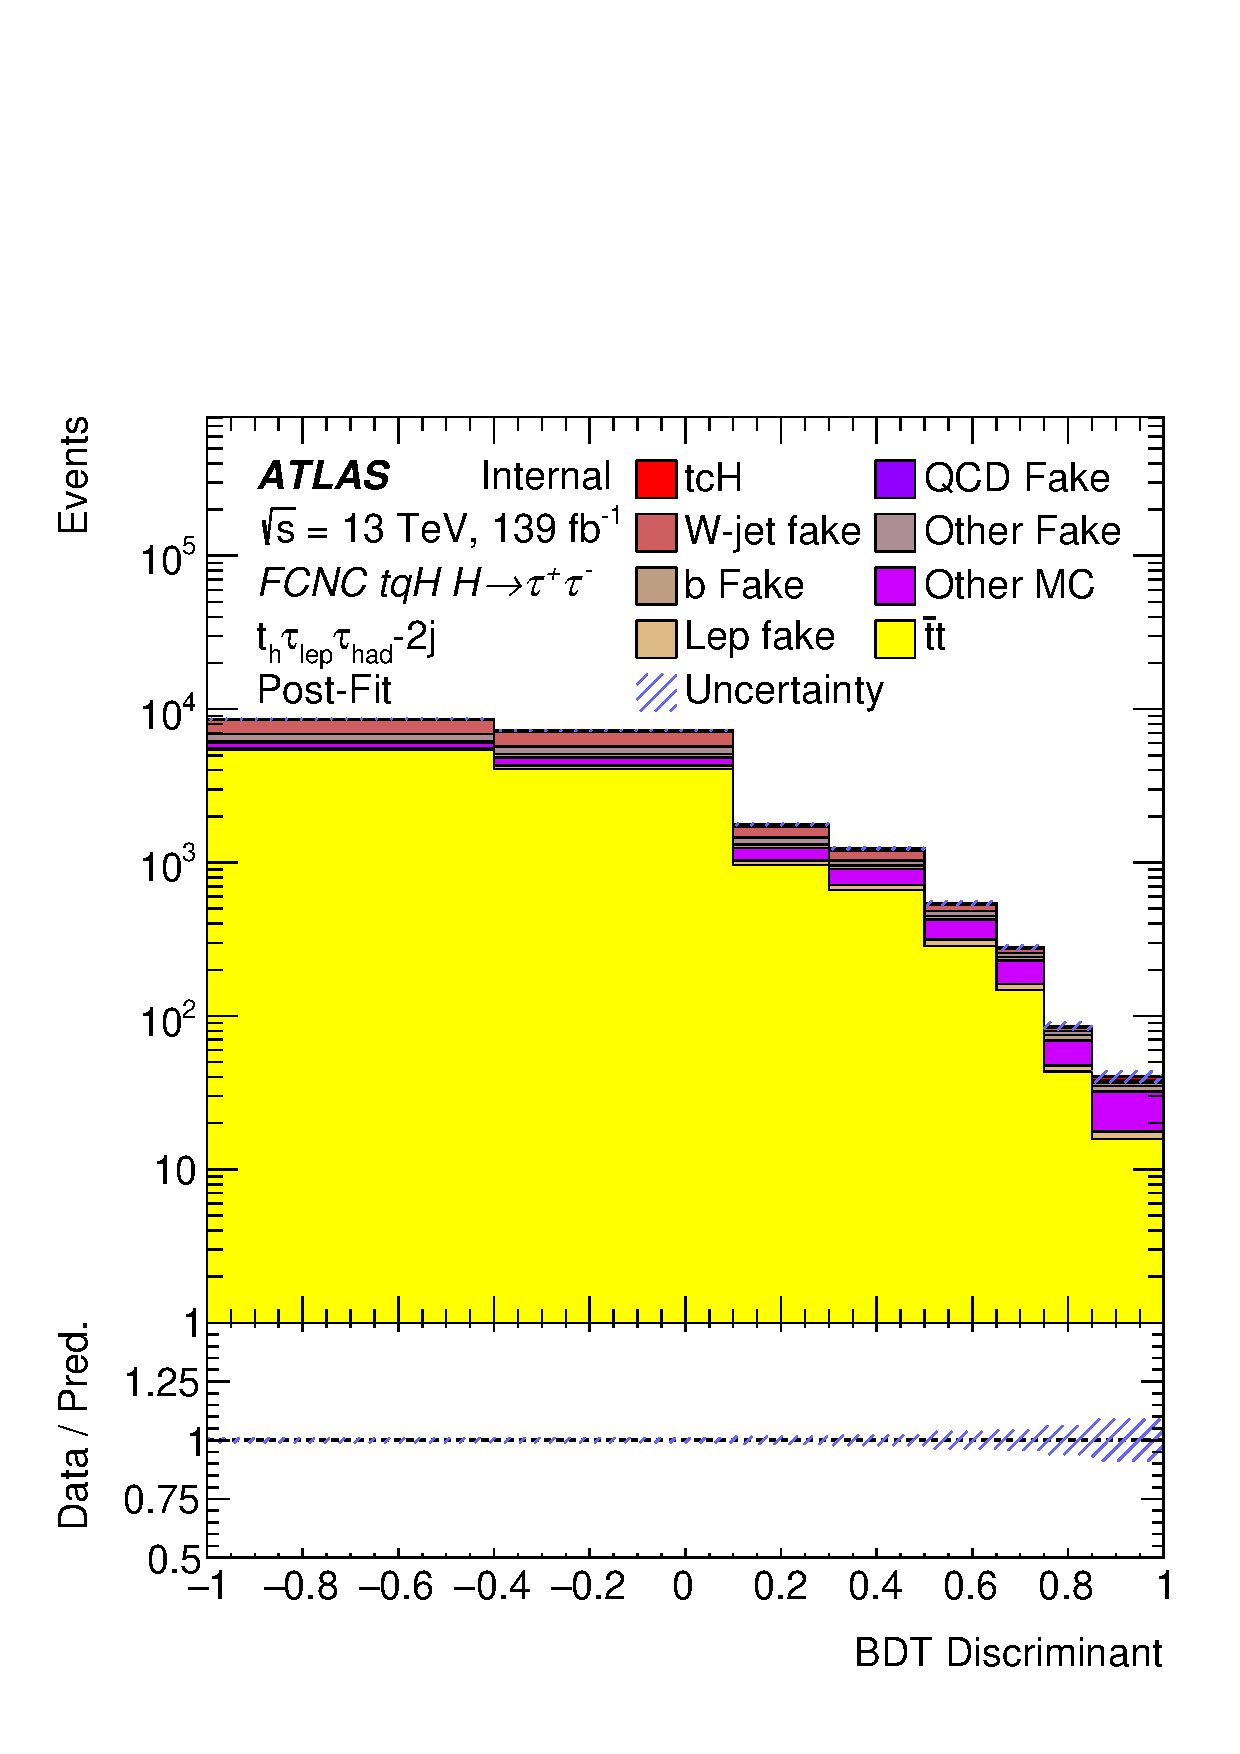
\includegraphics[width=0.40\textwidth]{\FCNCFigures/unblinded/ttHML/tcH_reg1l1tau1b2j_os_postFit.pdf}
\put(-100, 55){\textbf{(a2)}}\\
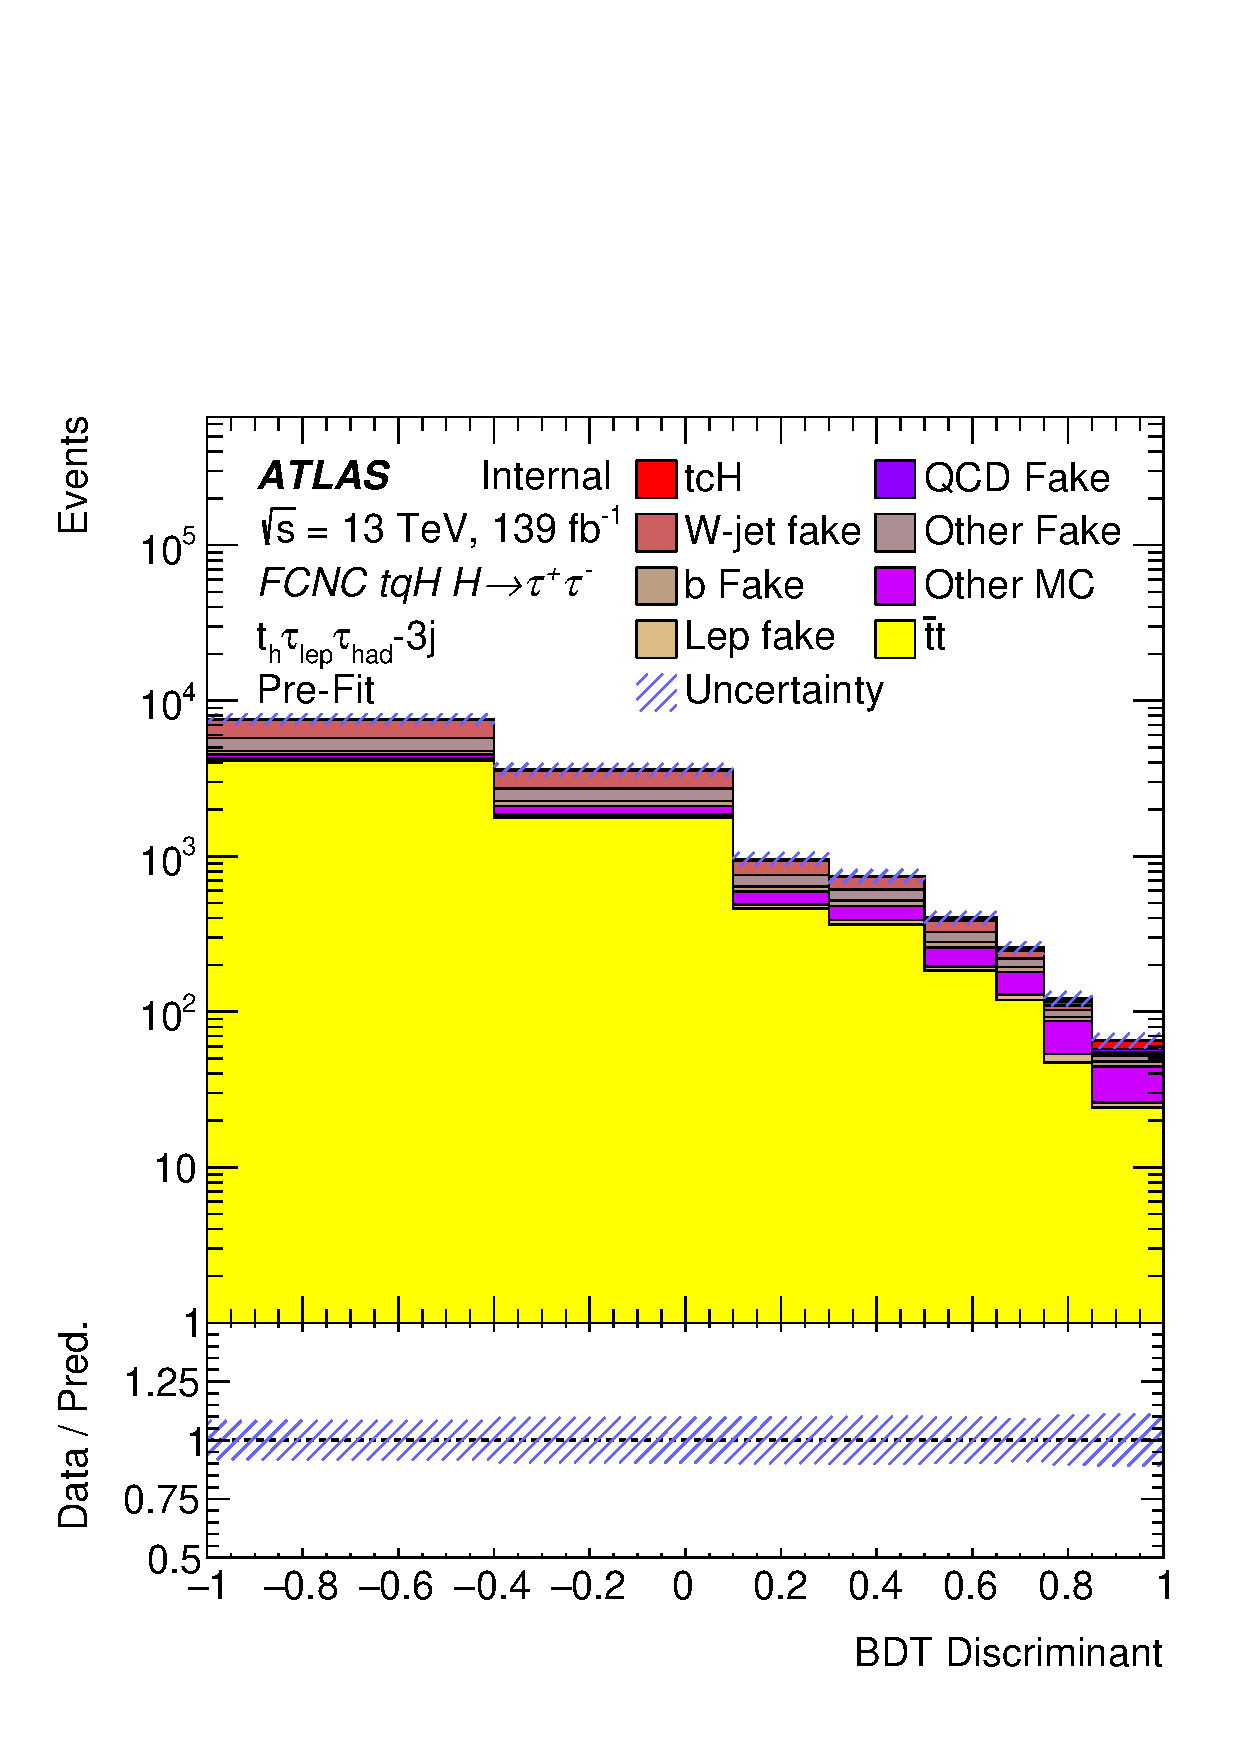
\includegraphics[width=0.40\textwidth]{\FCNCFigures/unblinded/ttHML/tcH_reg1l1tau1b3j_os.pdf}
\put(-100, 55){\textbf{(b1)}}
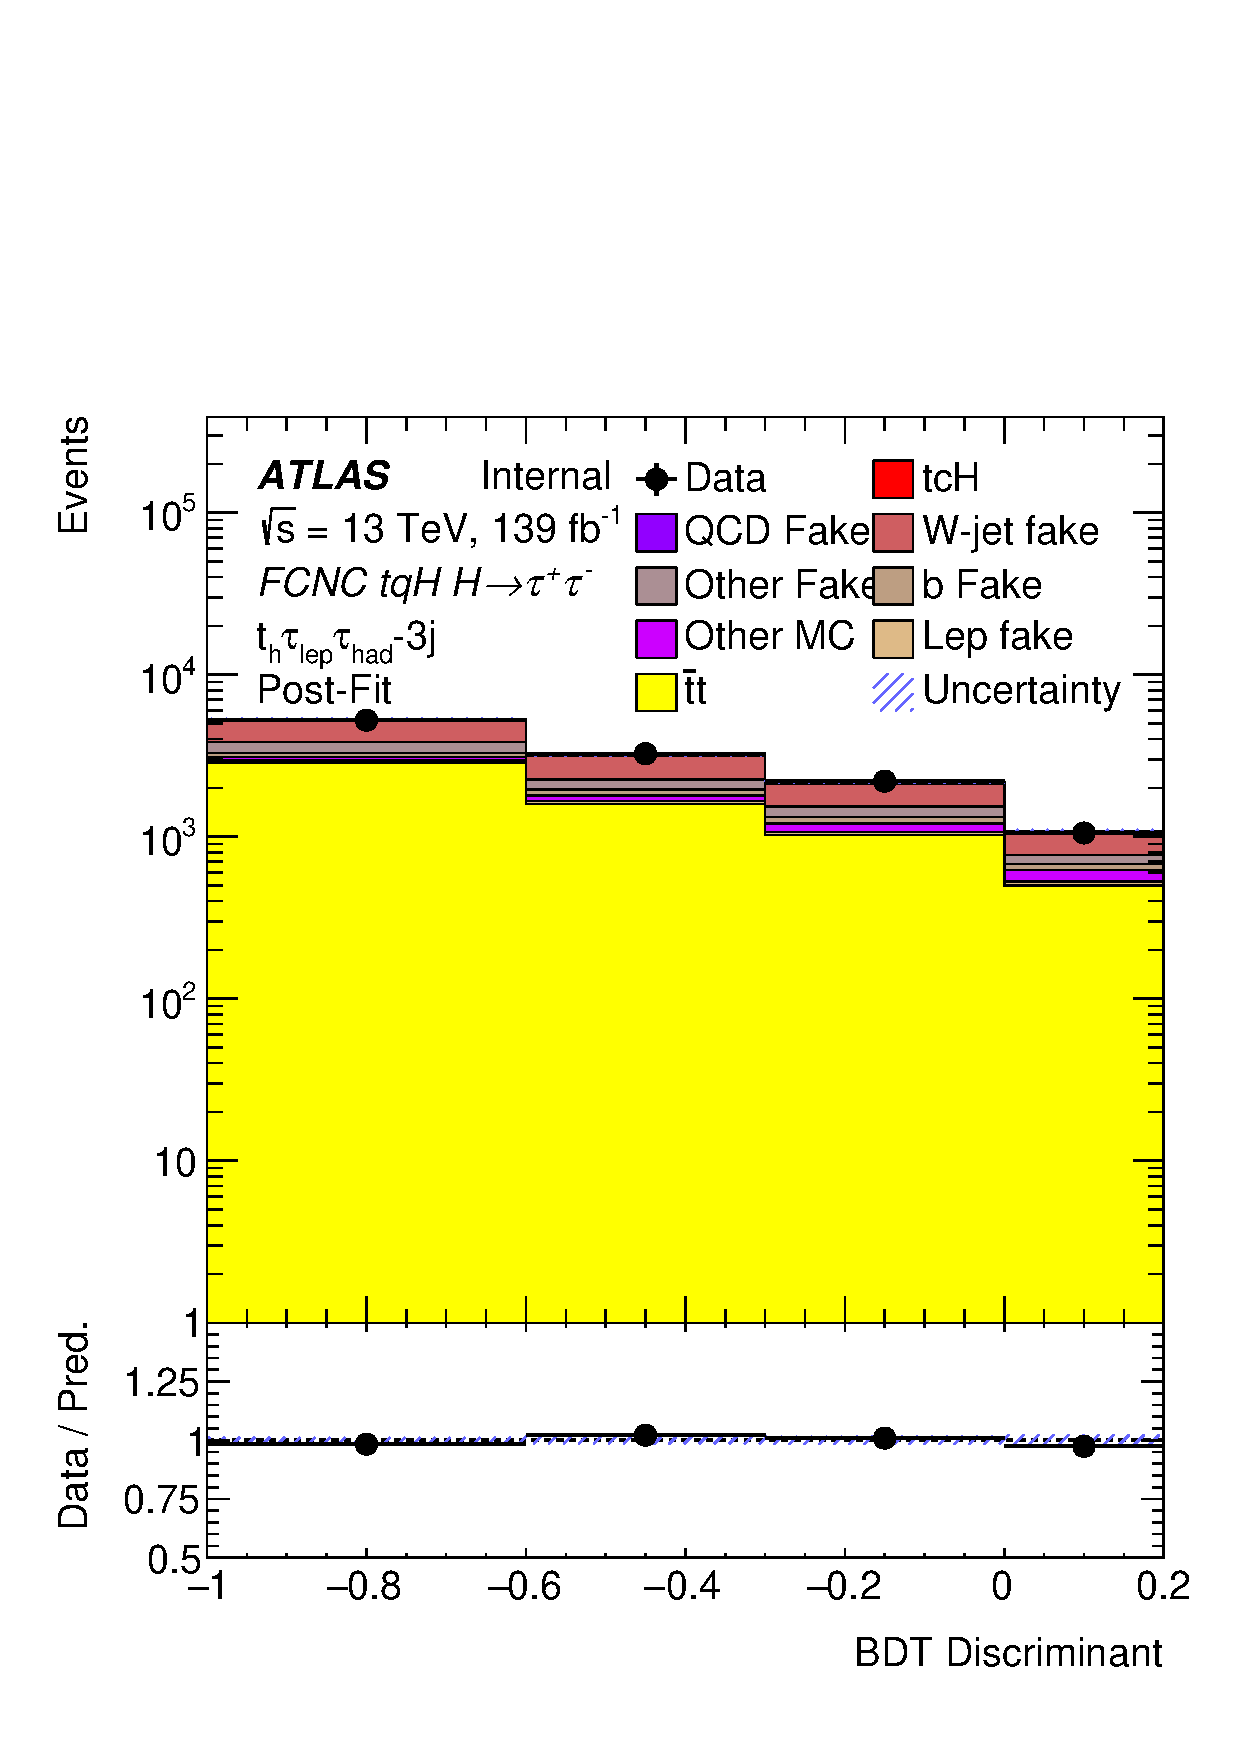
\includegraphics[width=0.40\textwidth]{\FCNCFigures/unblinded/ttHML/tcH_reg1l1tau1b3j_os_postFit.pdf}
\put(-100, 55){\textbf{(b2)}}\\
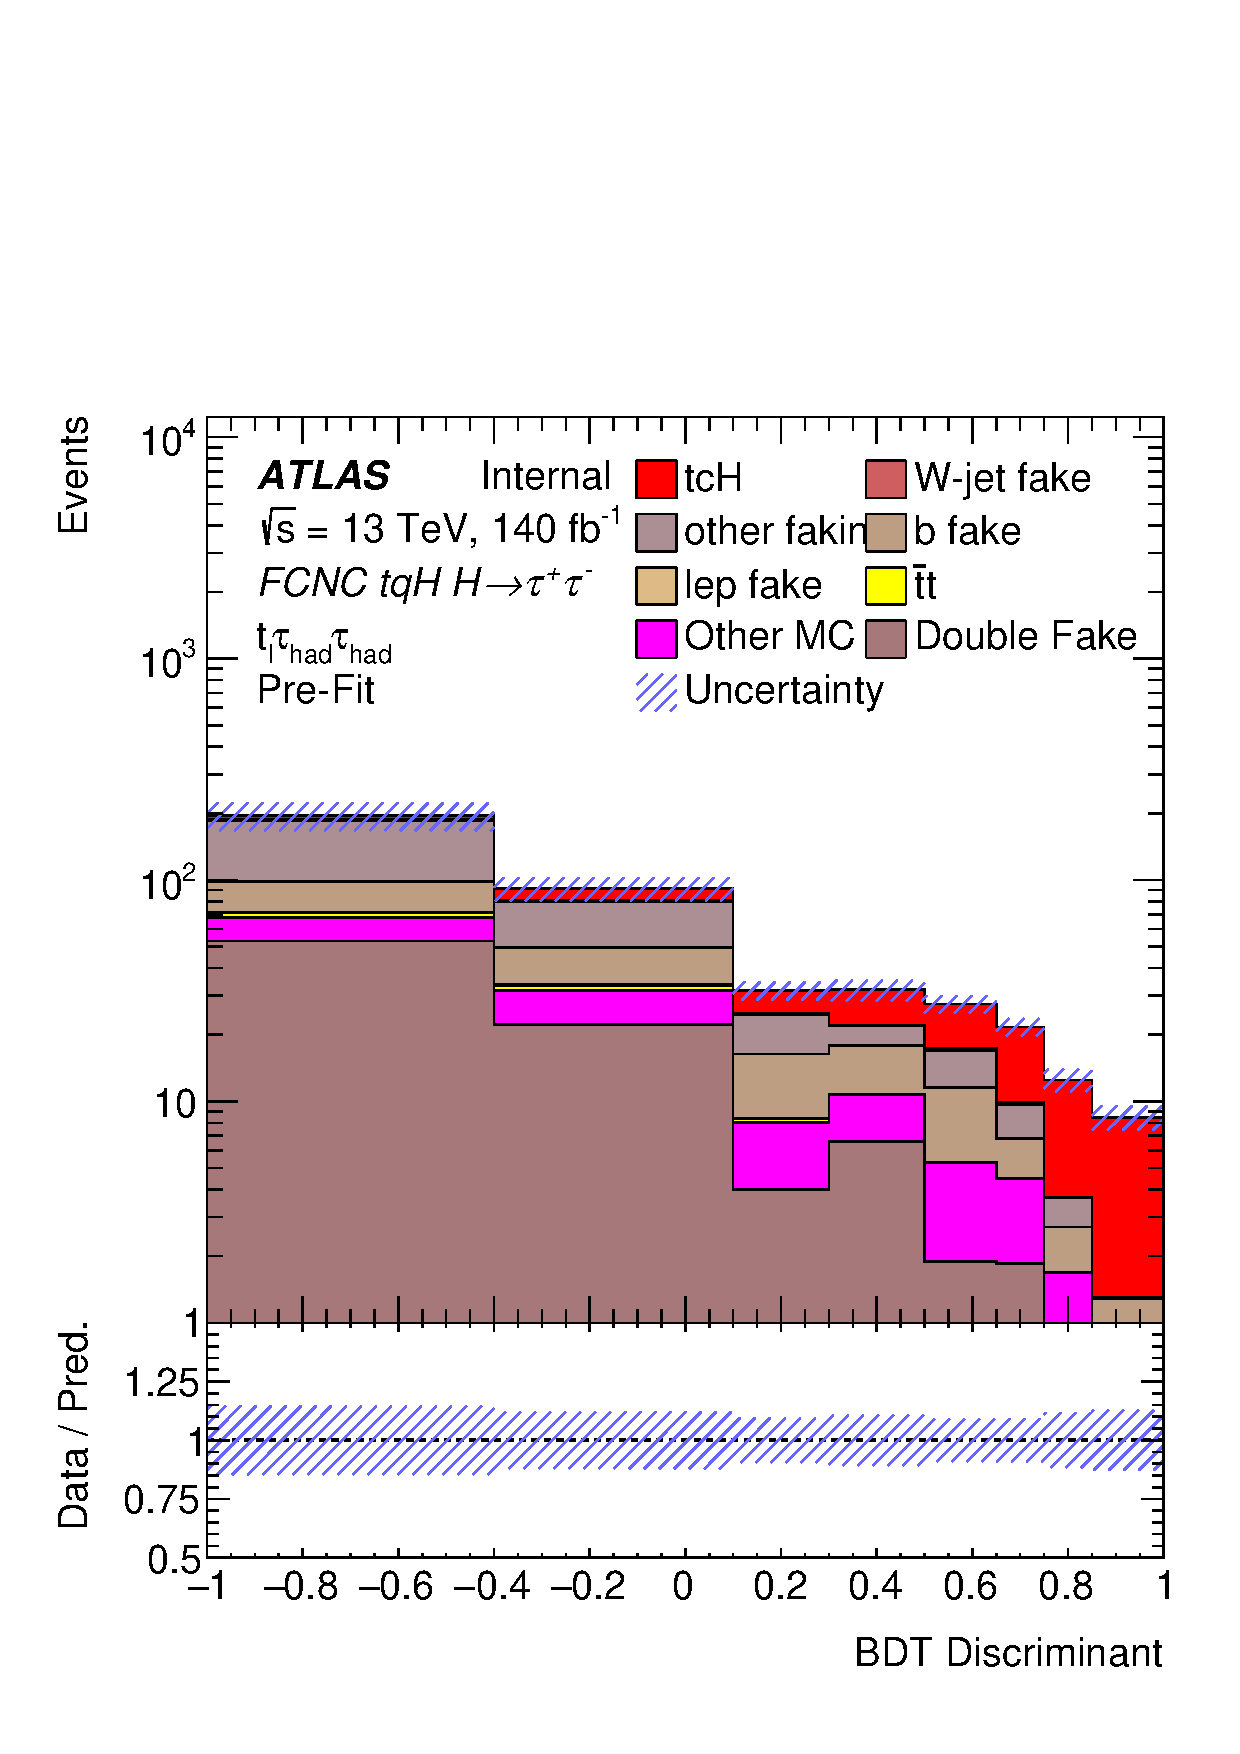
\includegraphics[width=0.40\textwidth]{\FCNCFigures/unblinded/ttHML/tcH_reg1l2tau1bnj_os.pdf}
\put(-100, 55){\textbf{(c1)}}
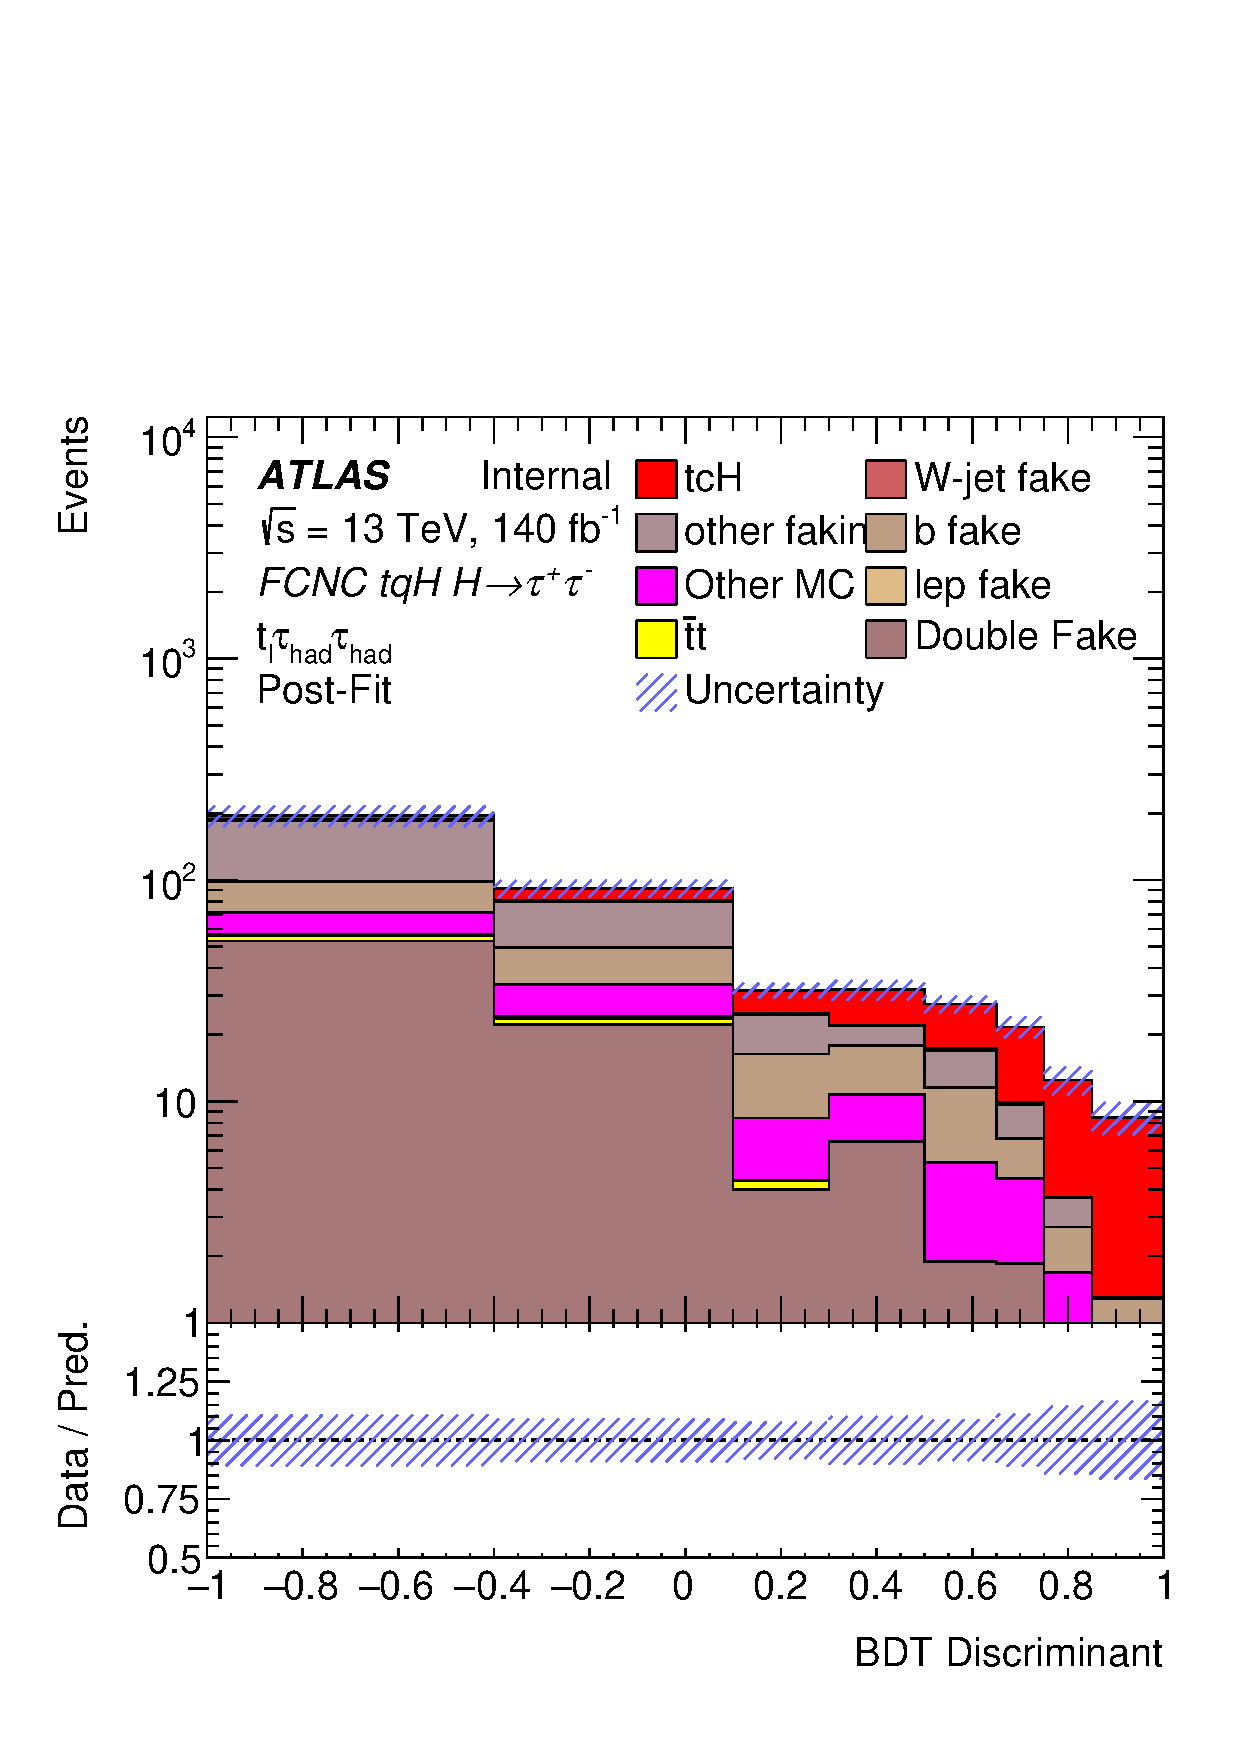
\includegraphics[width=0.40\textwidth]{\FCNCFigures/unblinded/ttHML/tcH_reg1l2tau1bnj_os_postFit.pdf}
\put(-100, 55){\textbf{(c2)}}\\

\caption{ Comparison of the shape of the BDT discriminant distribution between the unblinded prefit (a1,b1), unblinded postfit (a2,b2) in terms of tcH merged signal. The upper two plots are in the  $t_h\tlhad$-2j (a1-a2) region, the medium two are in $t_h\tlhad$-3j (b1-b2) and the bottom two are in $t_l\thadhad$ (c1-c2). Statistical and systematic uncertainties are being shown.}
\label{fig:tthML_trexPrefit_tcH}
\end{figure}

\begin{figure}[H]
\centering
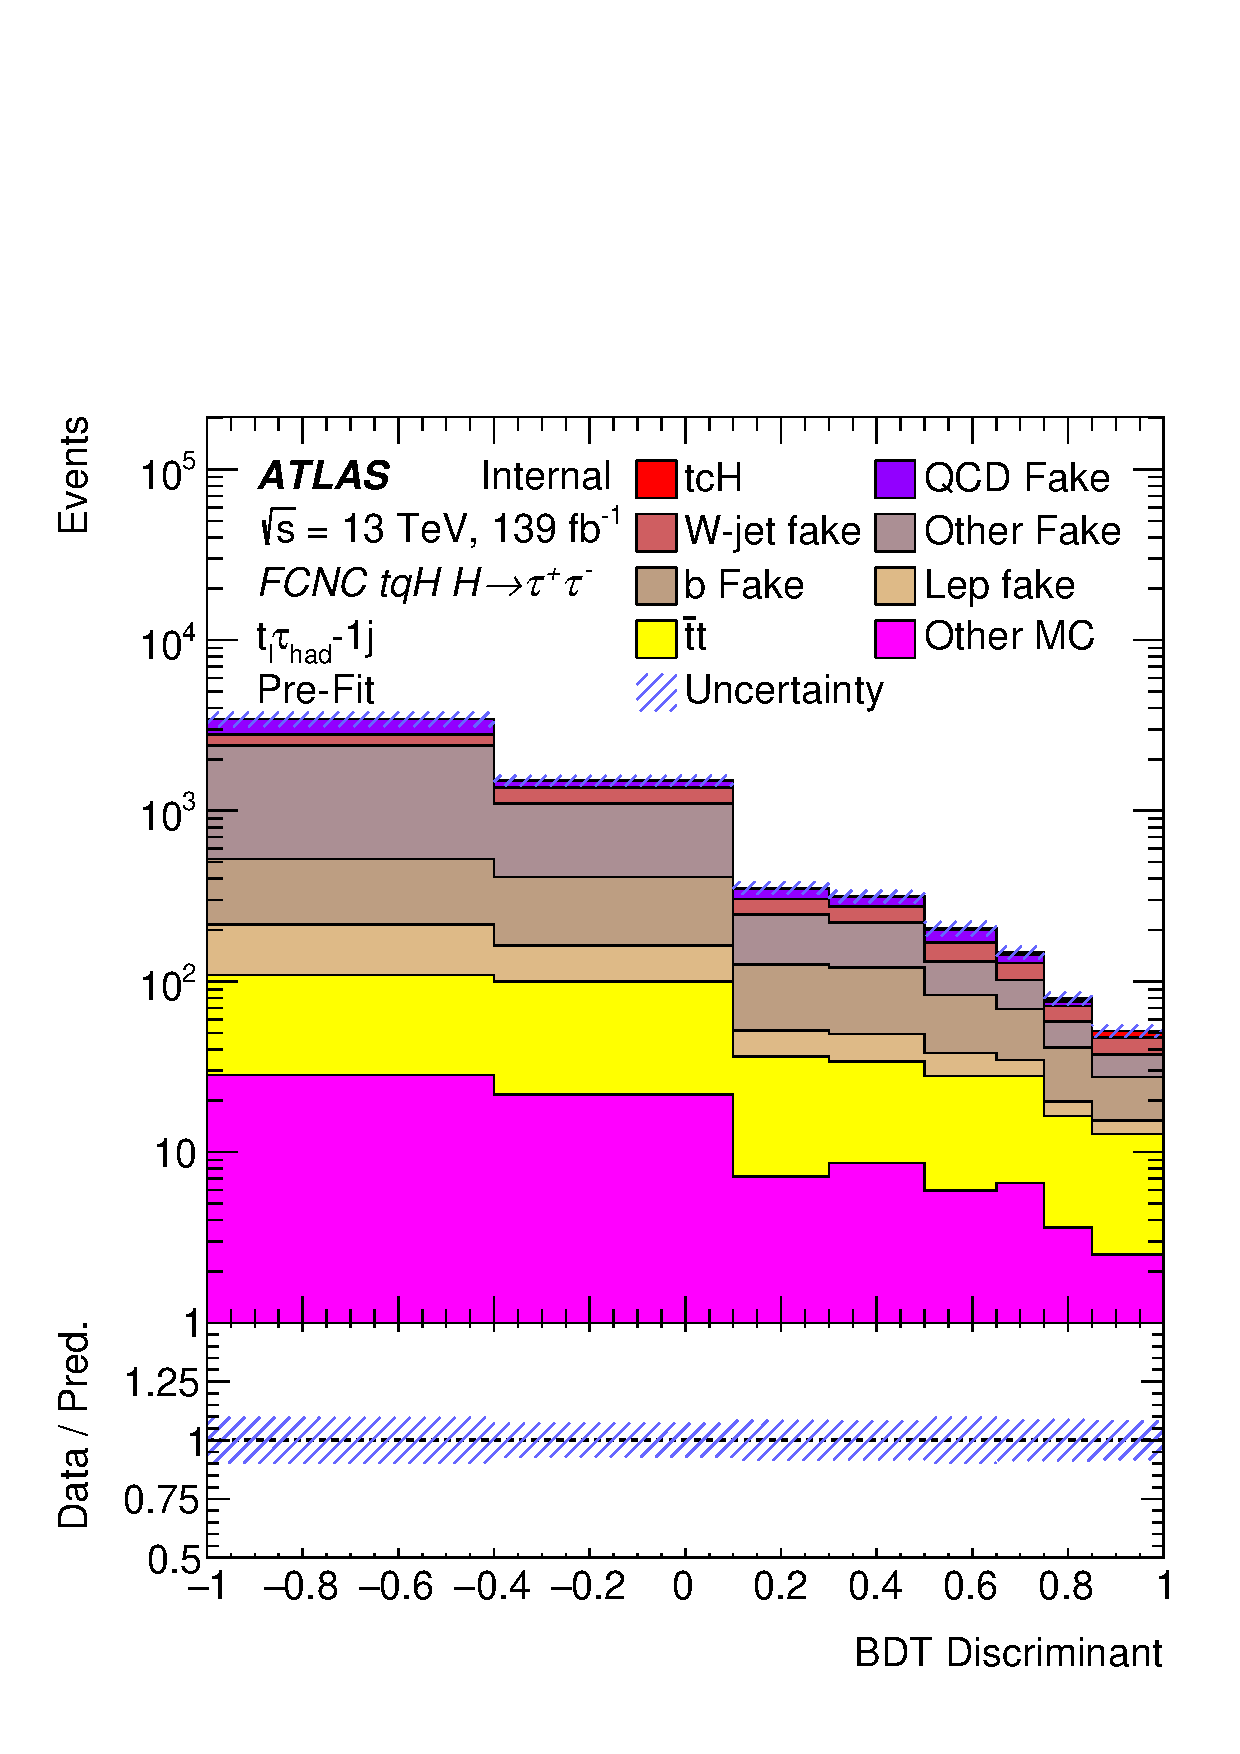
\includegraphics[width=0.50\textwidth]{\FCNCFigures/unblinded/ttHML/tcH_reg1l1tau1b1j_ss.pdf}
\put(-100, 55){\textbf{(a1)}}
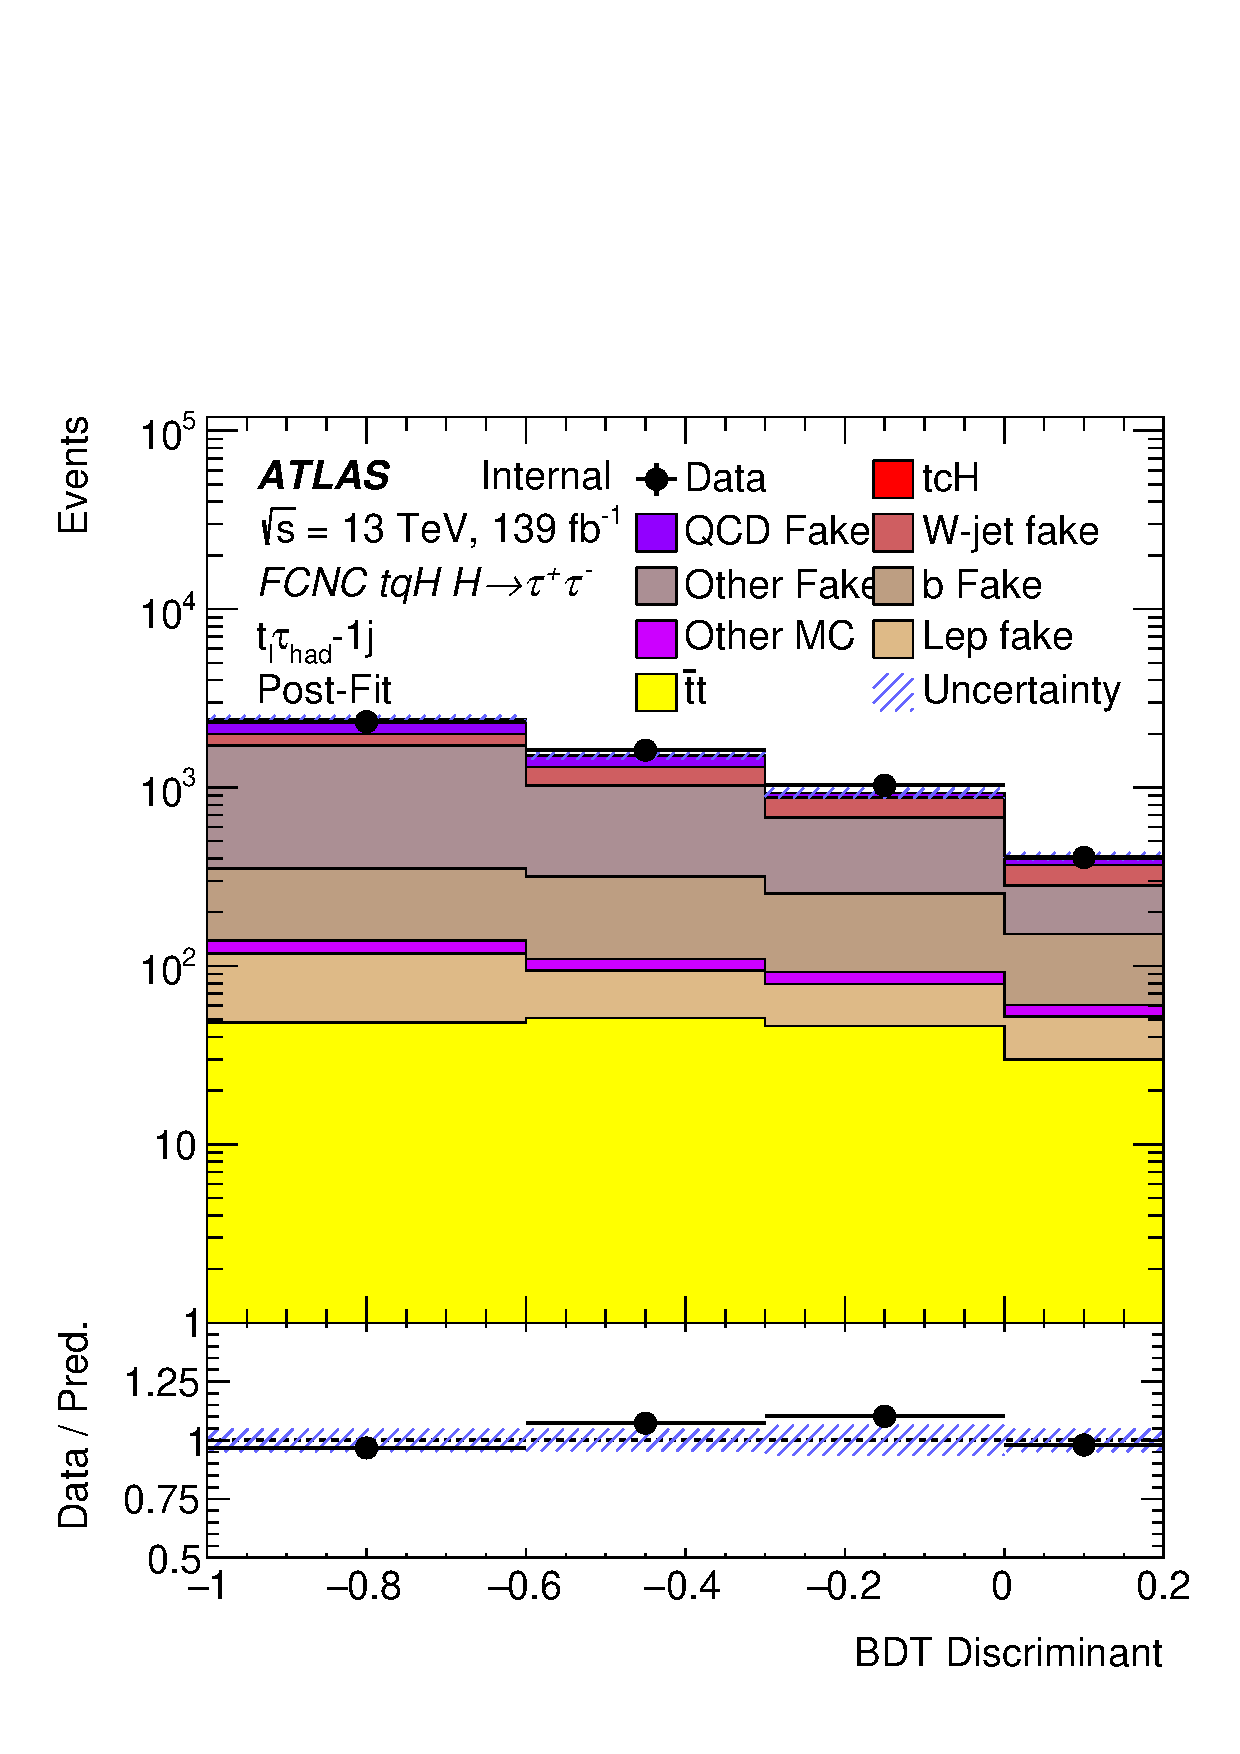
\includegraphics[width=0.50\textwidth]{\FCNCFigures/unblinded/ttHML/tcH_reg1l1tau1b1j_ss_postFit.pdf}
\put(-100, 55){\textbf{(a2)}}\\
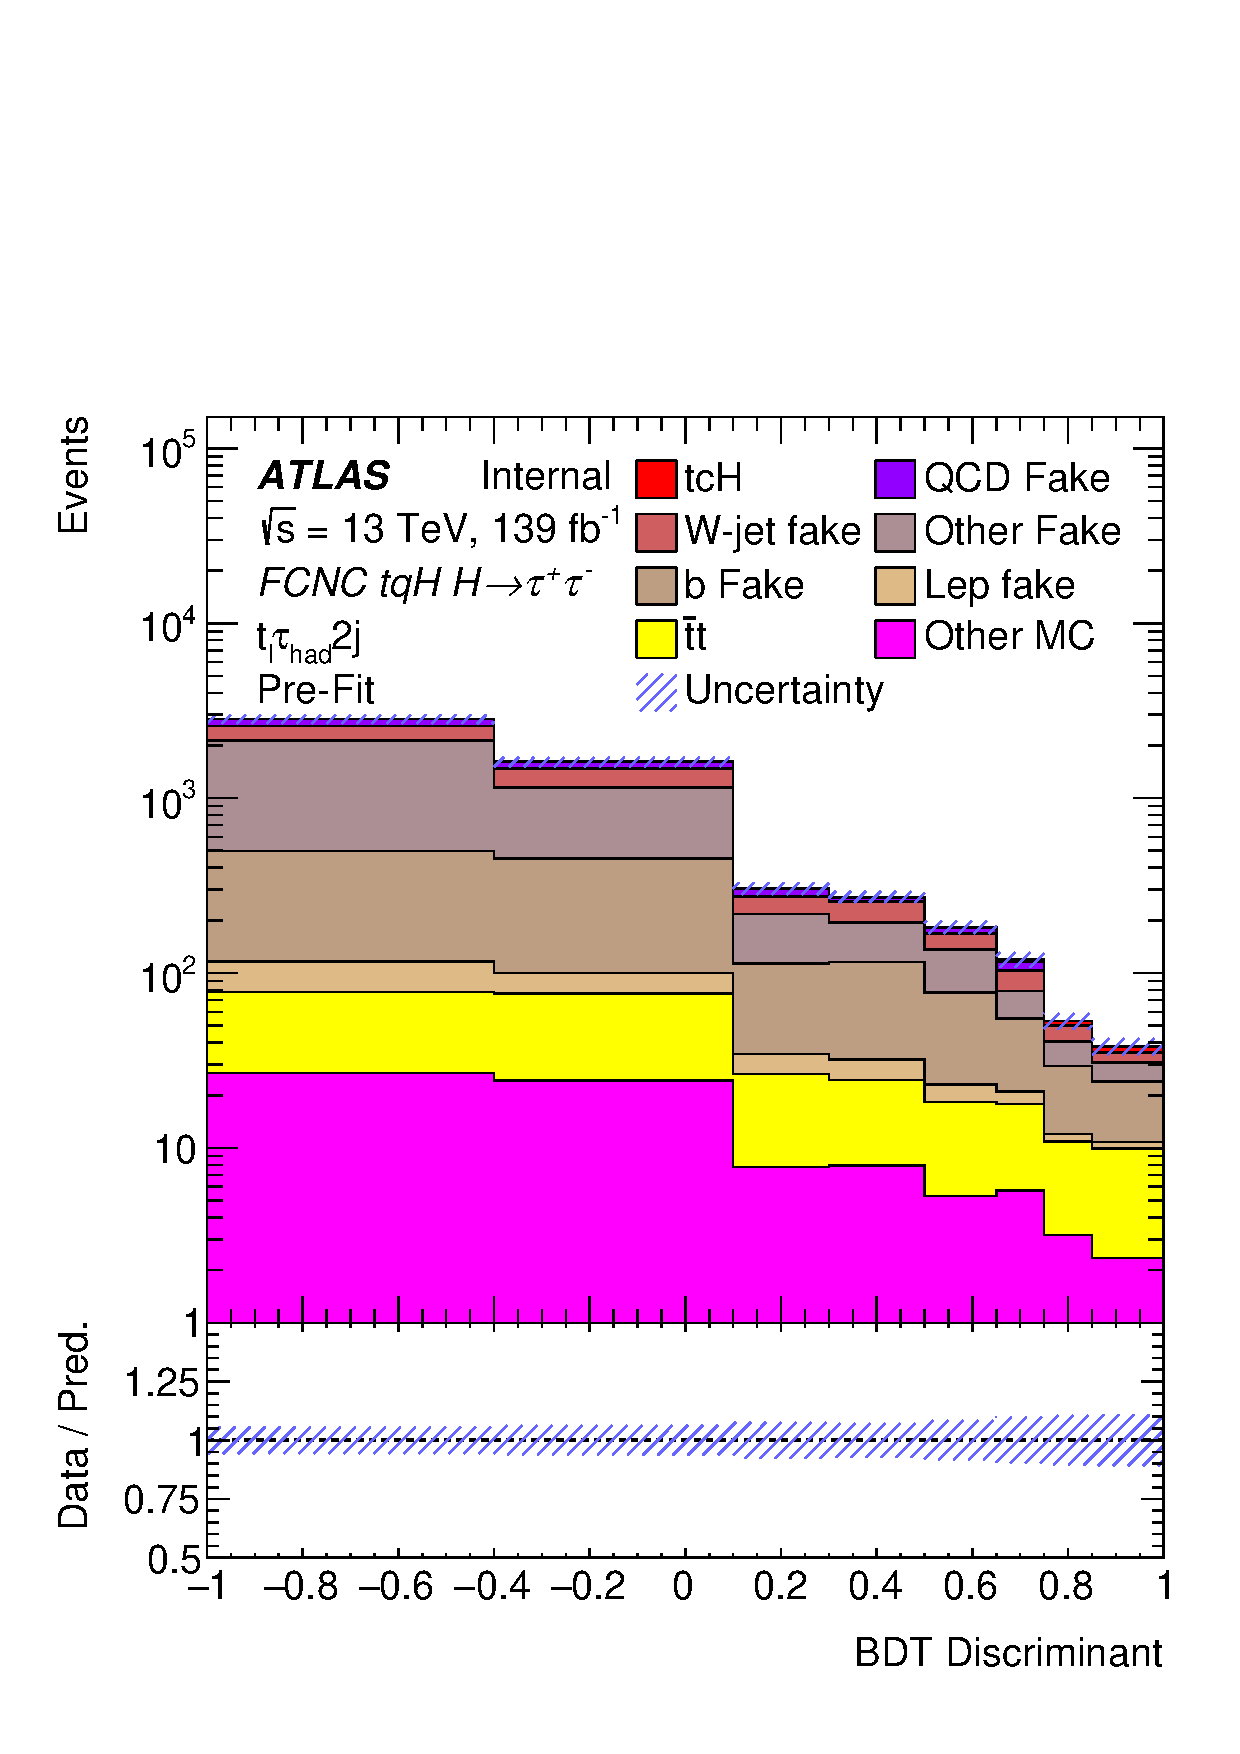
\includegraphics[width=0.50\textwidth]{\FCNCFigures/unblinded/ttHML/tcH_reg1l1tau1b2j_ss.pdf}
\put(-100, 55){\textbf{(b1)}}
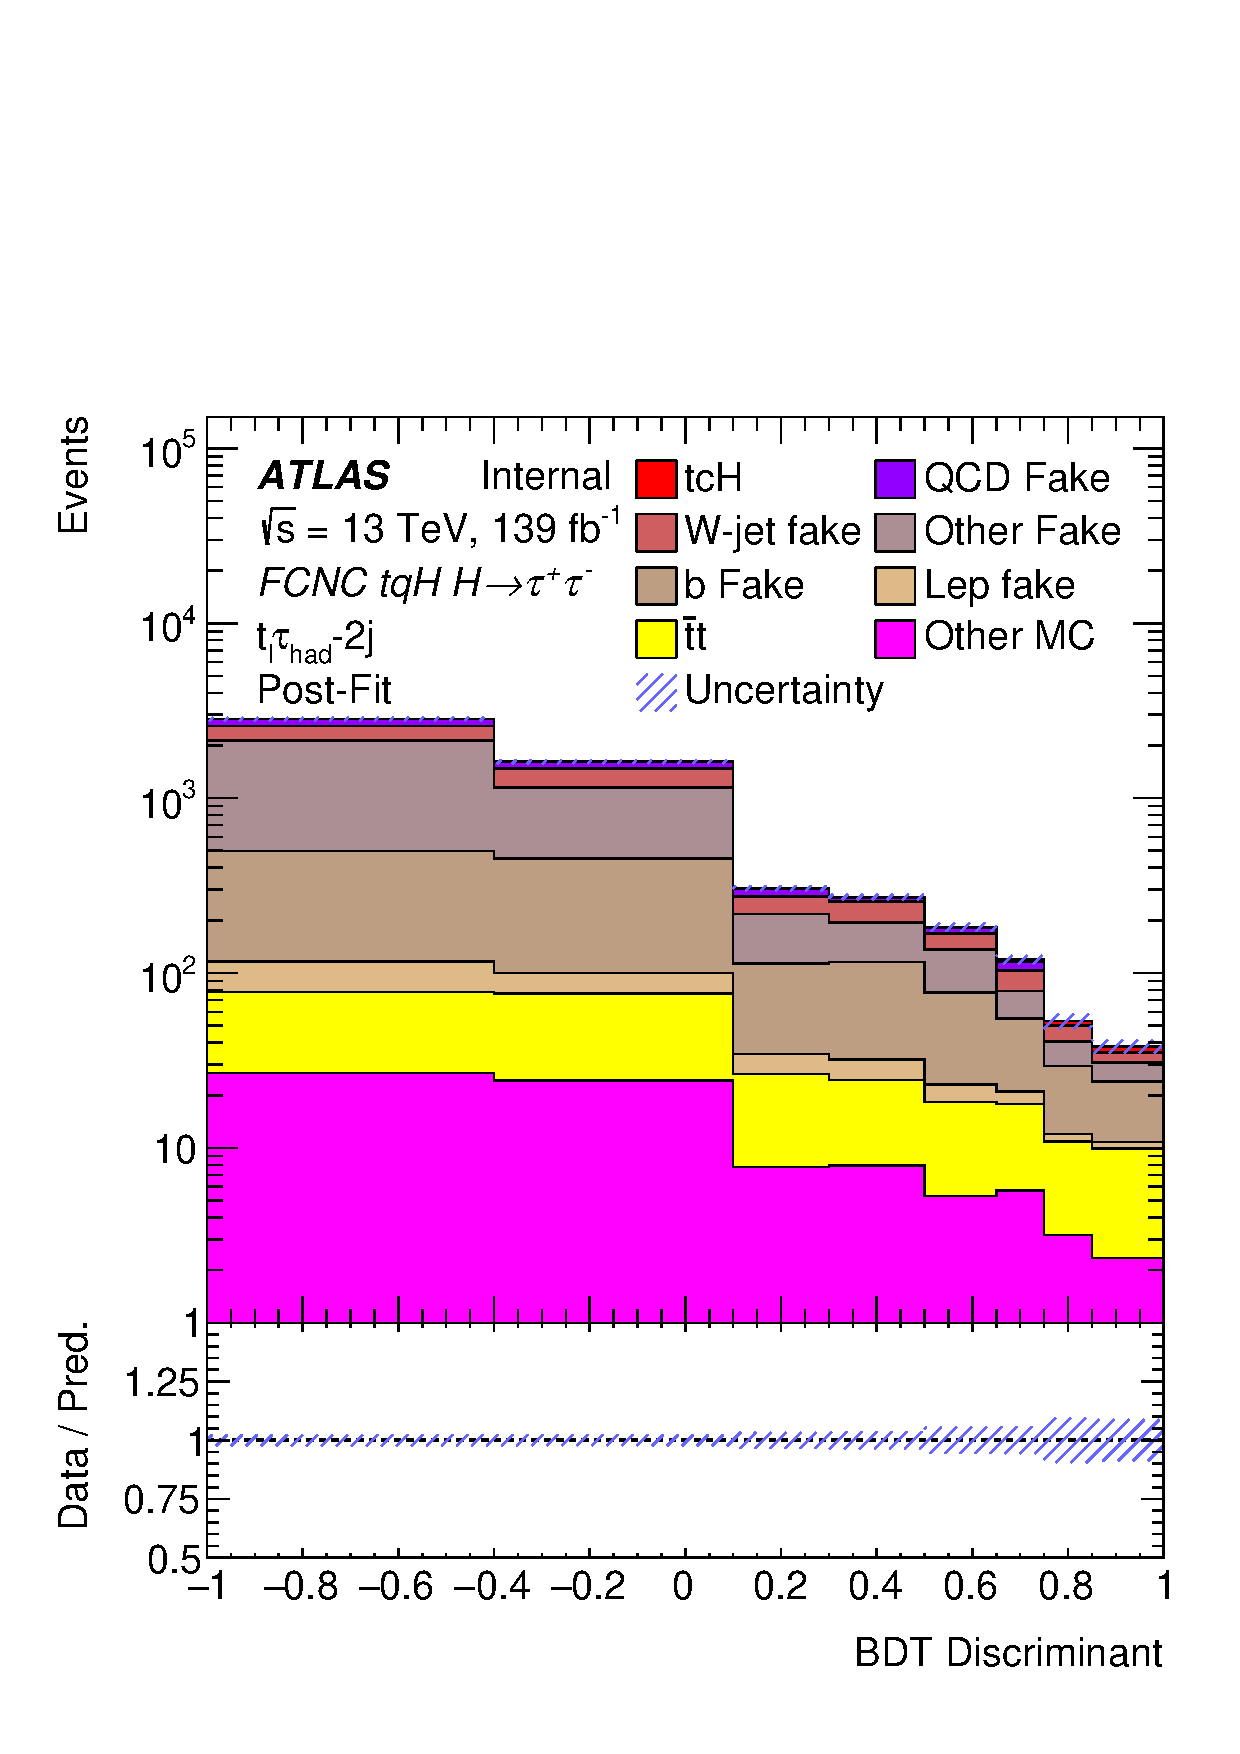
\includegraphics[width=0.50\textwidth]{\FCNCFigures/unblinded/ttHML/tcH_reg1l1tau1b2j_ss_postFit.pdf}
\put(-100, 55){\textbf{(b2)}}\\

\caption{ Comparison of the shape of the BDT discriminant distribution between the unblinded prefit (a1,b1), unblinded postfit(a2,b2) in terms of tcH merged signal. The upper two plots are in the  $t_l\tauhad$-1j (a1-a2) region, and the bottom two are in $t_l\tauhad$-2j (b1-b2).	Statistical and systematic uncertainties are being shown.}
\label{fig:tthML_trexPrefit_1_tcH}
\end{figure}
